\documentclass[a4paper, 12pt, diplomski]{etf}

\usepackage[intlimits]{amsmath}
\usepackage{amsmath, amsfonts, amssymb, graphicx}

\usepackage[serbian]{babel}
\usepackage[T1]{fontenc}
\usepackage[utf8]{inputenc}

\addto\captionsserbian{\renewcommand{\bibname}{Literatura}}

\title{Implementacija AXI periferije na FPGA čipu}
\author{Lazar Caković}
\indeks{256/2012}
\date{septembar 2016.}
\mentor{prof.~dr Lazar Saranovac}
\predmet{Namenski računarski sistemi}

\begin{document}

	\maketitle


	\begin{abstract}

		U ovom radu biće prikazana implementacija AXI periferije na FPGA (\textit{Field Programmable Gate Array}) čipu i njeno uključenje u veći računarski sistem korišćenjem kernela Linux-a. Sistem je realizovan u programskom paketu Vivado i SDK, proizvođača Xilinx. Periferija je implementirana u VHDL-u (\textit{VHSIC (Very High Speed Integrated Circuit) Hardware Description Language}). Program koji je potreban za korišćenje periferije implementiran je u \textit{C} programskom jeziku, neophodne skripte su implementirane u \textit{bash} jeziku, a aplikacija za sam sistem u \textit{shell} jeziku.

	\end{abstract}

	\begin{keywords}

		AXI, FPGA, Linux, embedded, Kernel, VHDL, C, bash, shell, software, hardware, driver, Xilinx, Vivado, SDK

	\end{keywords}

	\tableofcontents

	\listoffigures

	\newpage

	\chapter{Uvod}

		,,\textit{The industrial revolution appears as a knife-edge change from a rural self-employed lifestyle to a clock-punching, whistle-blowing corporate urban way of life. Being in the middle of the current revolution makes it hard to realize that in fifty years most people will consider the messy, dynamic, no-rules embedded product development environment of today as an obvious clean transition caused by technological changes.}``\cite{lit1}, Tod Fišer (\textit{Todd Fischer}, President and Founder, Cadenux).

		Integrisan sistem (embedded system) je računarski sistem specijalne namene koji je dizajniran da obavlja veoma male skupove aktivnosti. Integrisani sistemi se koriste od 1960-ih godina, gde su korišćeni za elektromehaničku kontrolu telefonskih centrala. Prvi poznatiji ugrađeni sistem je bio računar za navođenje u \textit{Apollo}, koji je razvio Čarls Drejper (\textit{Charles Draper}) i njegov tim. Kasnije su se integrisani sistemi proširili na vojnu, medicinsku, avio i automobilsku industriju. Danas su široko rasprostranjeni, i obavljaju ogroman broj funkcija. \cite{lit1}

		Kao što je navedeno, integrisani sistem ima za cilj da obavlja neke aktivnosti i da je uključen u neki veći kompjuterski sistem. Zamisao je da se napravi jedan sistem, koji će implementirati jednostavne stvari, ali koje će potpuno i pouzdano raditi taj mali set aktivnosti. Ovaj jednostavan integrisani sistem je zamišljen da radi uz pomoć kernela Linux-a. Osnovni razlog za korišćenje Linux-a je taj što je \textit{open source}, i ima mogućnosti izmene za korišćenje u svrhe embedded sistema. Sekundarni razlozi su ti da je Linux veoma dobro dokumentovan, kao i da iza korišćenja Linux-a u integrisanim sistemima postoji ogromna zajednica entuzijasta koja radi na njegovom unapređenju, kao i stvaranju integrisanih sistema.

		Implementirani sistem poseduje jedan uređaj koji je vrlo jednostavan, pored ostalih delova jednog kompjuterskog sistema. Cilj je da se pokaže jedan ceo proces, uz teorijsku osnovu i propratne komentare, od zamisli do realizacije i korišćenja uređaja, odnosno celog sistema. Periferija sistema je zamišljena kao AXI4-Lite, gde bi se prikazale mogućnosti AXI protokola. Za realizaciju je korišćena ploca ZC702, proizvođača Xilinx. Ovako zamišljena periferija može predstavljati deo jednog mnogo obimnijeg sistema, i na ovaj način se mogu implementirati mnogo komplikovaniji delovi sistema.

		U prvom poglavlju će biti prikazana hardverska realizacija samog sistema, nakon toga AXI (\textit{Advanced eXtensible Interface}) protokol koji je korišćen za implementaciju periferije unutar sistema, a zatim će biti dat opis Linux kernela i svih njegovih funkcionalnosti koje su bile potrebne za rad. I na kraju, softverska realizacija sistema, odnosno implementacija programa koji su bili neophodni kako bi sistem bio funkcionalan.	Kao i aplikacije koja predstavalja finalni proizvod koji korisnik treba da dobije uz uređaj.

		Rad je realizovan u kompaniji \textit{NovelIC} kao deo programa studentske prakse.

	\newpage

	\chapter{Hardverska realizacija}

	Sistem čije je projektovanje i korišćenje opisano u ovom radu je razvijan u hardverskom okruženju ZC702 proizvođača Xilinx. Ova ploča sa čipom XC7Z020 \textit{All Programmable SoC} (AP SoC) pruža hardversko okruženje za razvoj i testiranje sistema namenjenih za uređaj XC7Z020-1CLG484C. Ovo razvojno okruženje poseduje veliki broj mogućnosti za razvoj embedded (ugrađenih) procesorskih sistema. Između ostalog i DDR3 memoriju, Ethernet port sa tri moda rada, veliki broj I/O pinova opšte namene, dva UART(\textit{Universal asynchronous receiver/transmitter}) modula za komunikaciju sa spoljašnjim svetom, i td. Set ovih mogućnosti se može proširiti dodavanjem VITA-57 FPGA preko FMC (\textit{FPGA Mezzanine Card}) konektora koji se nalaze na ploči.\cite{lit2}

		\begin{figure}[htb]
			\centering
			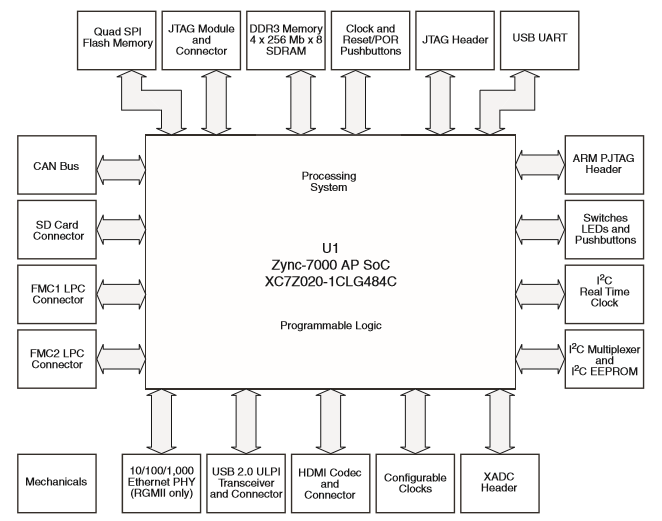
\includegraphics[width=.6\textwidth]{images/zynq7000APSoC.png}
			\caption{Blok dijagram XC7Z020 AP SoC}
			\label{fig:zynq}
		\end{figure}

	Neke od mogućnosti su prikazane na slici \ref{fig:zynq}.

	Razvojna ploča poseduje određen broj prekidača, dugmadi i dioda koje služe za testiranje. Naravno, ukoliko to nije dovoljno, uvek se preko različitih načina komunikacije može povezati veliki broj periferija koje mogu poslužiti testiranju.
ZC702 kao što je navedeno, sadrži Zynq-7000 XC7Z020-1CLG484C AP SoC (\textit{All Programmable System On Chip}). XC7Z020 AP SoC se sastoji od procesorskog sistema (PS – processing system) i programabilne logike (PL – programmable logic) na jednom čipu. Procesorski sistem integriše dva ARM® Cortex™-A9 MPCore™ procesora, AMBA® interkonekciju, interne memorije, interfejse ka eksternim memorijama, i periferije koje uključuju USB, Ethernet, SPI, SD/SDIO, I2C, CAN, UART, i GPIO.\cite{lit2} Procesorski sistem radi nezavisno od programabilne logike i pokreće se po uključenju sistema ili nakon reseta cele ploče.

		\begin{figure}[htb]
			\centering
			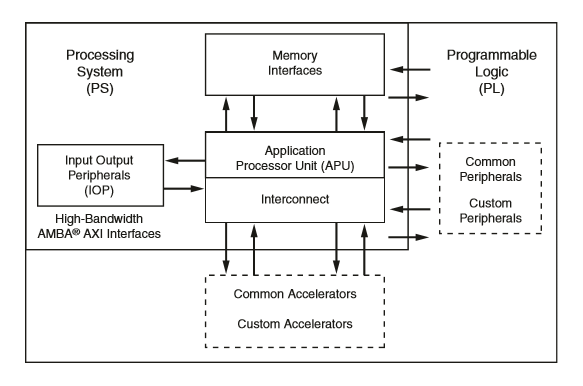
\includegraphics[width=.7\textwidth]{images/PSZYNQ7000.png}
			\caption{Blok dijagram procesorskog sistema i programabilne logike}
			\label{fig:procSysProgLog}
		\end{figure}

	Čip Zynq-7000 AP SoC je vrlo komplikovan i ima mnogo mogućnosti, što se može videti na slici \ref{fig:zynqBlock} koji predstavlja ceo čip sa svim njegovim mogućnostima.

		\begin{figure}[htb]
			\centering
			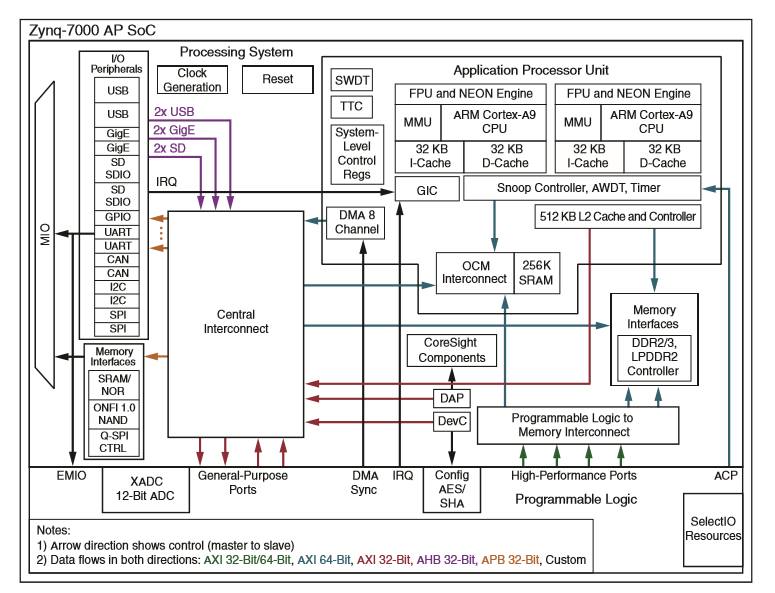
\includegraphics[width=.6\textwidth]{images/ZYNQ7000BD.png}
			\caption{Blok dijagram celog čipa}
			\label{fig:zynqBlock}
		\end{figure}

	Ovo razvojno okruženje koristi proces inicijalizacije sistema iz više faza koji podržava način i nesigurne i sigurne inciijalizacije. U ovom slučaju procesorski sistem čipa je master, ali i konfiguracionog procesa. ZC702 ploča podržava sledeće konfiguracije:

	\begin{itemize}

		\item Konfiguracija procesorskog sistema: Quad SPI flash memory
		\item Konfiguracija procesorskog sistema: Inicijalizacija procesorskog sistema sa SD memorijske kartice
		\item Konfiguracija programabilne logike: konfiguracija preko USB JTAG porta (Digilent module)
		\item Konfiguracija programabilne logike: konfiguracija preko JTAG porta

	\end{itemize}

	Izbor načina konfiguracije se bira podešavanjem stanja određenih prekidača na ploči.

	Ovaj sistem je u osnovi zamišljen kao veoma jednostavan, ali sa takvim osobinama da iskoristi potencijal čipa ZYNQ 7000, kao i pojedinim delovima ploče koji služe za testiranje. Razvoj hardverskog dela sistema realizovan je u Xilinx alatima Vivado i SDK.

	\newpage

	\chapter{AXI}

	Advanced eXtensible Interface (AXI) je deo ARM AMBA(Advanced Microcontroller Bus Architecture) familije magistrala za mikrokontrolere koji su prvi put uvedene 1996. godine. Prva verzija AXI je uključena u AMBA 3.0, koji je predstavljen 2003. godine. AMBA 4.0, predstavljen 2010. godine, uključuje drugu verziju AXI, AXI4 koja je i korišćena u izradi ovog sistema. Xilinx je usvojio AXI protokol za razvijanje svojih IP (IP - Intellectual Property) i to prvi put kada su uvedeni čipovi Spartan-6 I Virtex-6. \cite{lit3}

	AMBA AXI protokol podžava izradu sistema visokih performansi i visokih frekvencija. AXI protokol je idealan za projektovanje sistema visokog propusnog opsega i sistema sa malim kašnjenjem,  pruža mogućnost korišćenja operacija sa visokim frekvencijama. Naime, ovaj tip protokola je modularan za interfejse, i može se koristiti po sopstvenoj volji, kao i za memorijske kontrolere sa inicijalno velikim kašnjenjem pristupa. Mogućnosti AXI protokola su ogromne.

	Trenutno postoje tri tipa interfejsa koji rade sa AXI4 protokolom:

	\begin{itemize}

		\item AXI4 – za potrebe memorijski mapiranih uređaja visokih performansi.
		\item AXI4-Lite – za jednostavnu memorijski mapiranu komunikaciju (kao na primer za čitanje i upis u statusne i kontrolne registre).
		\item AXI4-Stream – za obradu podataka koji dolaze velikom brzinom.

	\end{itemize}

	AXI4 omogućava unapređenje i povećanje mogućnosti koje imaju Xilinx uređaji, i to u segmentima produktivnosti, fleksibilnosti i dostupnosti:

	\begin{itemize}

		\item Produktivnost – Standardizovanjem AXI interfejsa, inženjeri koji razvijaju sisteme mogu to raditi ukoliko znaju samo jedan protokol za IP.
		\item Fleksibilnost – Pružajući pravi protokol za aplikaciju koja je potrebna:

			\begin{itemize}

			\item AXI4 je za memorijski mapirane interfejse i omogućava burst mod rada od 256 prenosa podataka sa samo jednom adresnom fazom u protokolu.
			\item AXI4-Lite je za jednostavne, memorijski mapirane interfejse koji prenose samo po jedan podatak u jednom ciklusu. Vrlo je jednostavan, kako u dizajniranju sistema, tako i u korišćenju.
			\item AXI4-Stream nema potrebu za adresnom fazom unutar protokola, na osnovu čega podržava neograničenu veličinu burst moda. AXI4-Stream interfejsi se ne smatraju memorijski mapiranim, upr\-avo zbog nepostojanja adresne faze unutar protokola. Ovaj tip interfejsa je pogodan za protočnu obradu podataka.

			\end{itemize}


		\item Dostupnost – Prelazeći na industrijske standarde, dobija se pristup svim katalozima IP od ARM partnera, kao i katalozima Xilinx.

	\end{itemize}

	\section{Arhitektura}

	Svaka transakcija između mastera i slejva ima adresu i kontrolnu informaciju na adresi kanala koji opisuje prirodu podatka koji će se preneti, odnosno razmeniti. Podaci se prenose između mastera i slejva koristeći kanal za pisanje podataka do slejva, ili kanal za čitanje podataka do mastera. U procesu pisanja, u kome je ceo prenos podataka od mastera do slejva, ovaj protokol ima dodatni kanal za slanje odgovora na pisanje kako bi omogućio slejvu da dojavi masteru o završetku transakcije pisanja.

	AXI protokol omogućava:

	\begin{itemize}

		\item Da se informacija o adresi izda pre stvarnog prenosa podataka.
		\item Podršku za simultane nezavšene prenose podataka.
		\item Podršku za neispravne završetke prenosa podataka.

	\end{itemize}

	\begin{figure}[htb]
		\centering
		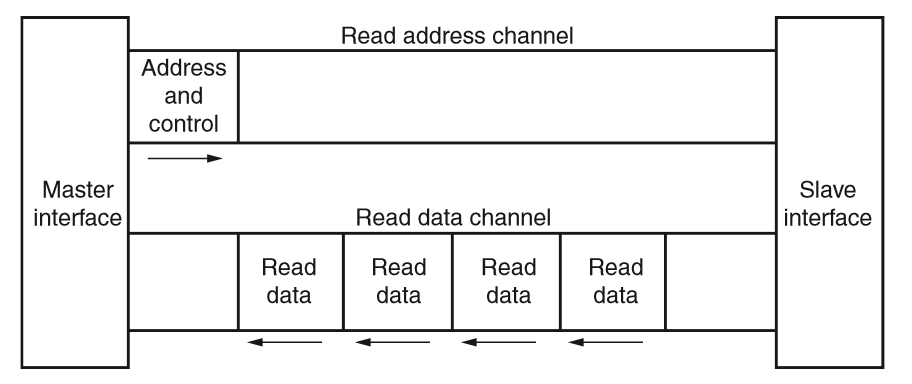
\includegraphics[width=.7\textwidth]{images/axireadprotocol.png}
		\caption{Protokol čitanja}
		\label{fig:axiread}
	\end{figure}

	Na slici \ref{fig:axiread} je prikazan proces čitanja koji koristi kanale za čitanje i adrese i podataka.

	\begin{figure}[htb]
		\centering
		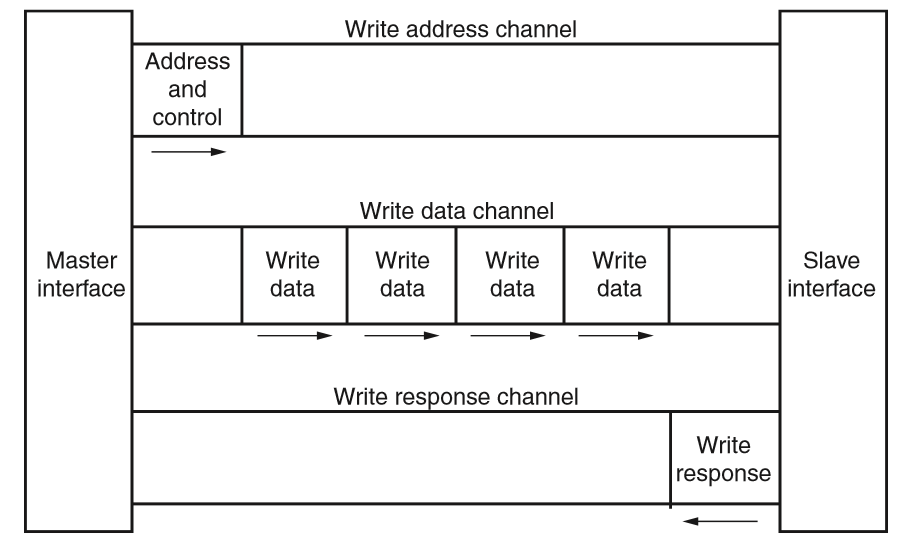
\includegraphics[width=.7\textwidth]{images/axiwriteprotocol.png}
		\caption{Protokol pisanja}
		\label{fig:axiwrite}
	\end{figure}

	Na slici \ref{fig:axiwrite} je prikazan proces pisanja koji koristi kanale za pisanje adrese, pisanje podataka, i pisanje odgovora masteru.

	Svaki od pet nezavisnih kanala se sastoji od seta informacionih signala i koristi dvosmerne \textit{VALID} i \textit{READY} mehanizme rukovanja (handshake mechanism). Izvor informacije u komunikaciji koristi \textit{VALID} signal kako bi pokazao da je podatak ili kontrolna informacija dostupna na kanalu, odnosno da je validna. Dok destinacija, odnosno onaj uređaj koji treba da primi tu informaciju koristi \textit{READY} signal kako bi pokazao da je u mogućnosti da primi informaciju koja mu je prosleđena. Kanali za pisanje i čitanje podataka uključuju i signal \textit{LAST} koji signalizira prenos poslednjeg podatka.

	\begin{itemize}

		\item Kanali za pisanje i čitanje adresa : Transakcije pisanja i čitanja imaju sopstvene adresne kanale. Odgovarajući adresni kanal nosi sve potrebne adrese i kontrolne informacije koje su potrebne kako bi se prenos informacija u potpunosti obavio.
		\item Kanal za čitanje podataka : Ovaj kanal obavlja kako čitanje podataka, tako i čitanje povratne informacije od slejva do mastera, pri čemu sadrži magistralu podataka koja može biti široka 8, 16, 32, 64, 128, 256, 512 ili 1024 bita, kao i odgovor koji ukazuje na završetak procesa čitanja.
		\item Kanal za pisanje podataka : Ovaj kanal obavlja pisanje podataka od mastera do slejva i uključuje magistralu podataka koja može biti široka 8, 16, 32, 64, 128, 256, 512 ili 1024 bita i jednu liniju od jednog bajta na svakih 8 bita podatka koji se prenosi, koja ukazuje na to koji su podaci validni. Informacije o kanalu za pisanje podataka su uvek tretirane kao baferisane, da bi master mogao da obavlja procese pisanja bez potrebe da slejv ima uvid u prethodne procese pisanja podataka.
		\item Kanal za pisanje odgovora : Ovaj kanal služi samo kao način da slejv dostavi odgovor masteru o završetku procesa pisanja. I svi procesi pisanja koriste signaliziranje za kraj jednog ciklusa. Ovaj signal za kraj se dešava jednom za svaki burst podataka, ali ne i za svaki prenos podataka unutar jednog bursta.

	\end{itemize}

\section{AXI sistem}

	Jedan tipičan sistem se sastoji od određenog broja uređaja koji predstavljaju master u nekoj komunikaciji, i određenog broja uređaja koji predstavljaju slejv. Uređaji su povezani preko dela sistema koji služi samo za interkonekciju ovih uređaja. AXI protokol omogućava jedinstvenu definiciju interfejsa, i to:

	\begin{itemize}

		\item Između mastera i dela za interkonekciju.
		\item Između slejva i dela za interkonekciju.
		\item Između mastera i slejva.

	\end{itemize}

	Definicija interfejsa omogućava paletu različitih implementacija dela za interkonekciju. Deo sistema koji je zadužen za interkonekciju, odnosno lokalnu komunikaciju između pojedinih uređaja se može smatrati kao poseban uređaj koji ima simetrične master i slejv portove preko kojih stvarni master i slejv uređaji mogu biti povezani.
	Većina sistema koristi jedan od tri načina za realizaciju dela za interkonekciju, i to:

	\begin{itemize}

		\item Deljena adresna magistrala i magistrala podataka.
		\item Deljena adresna magistrala i višestruka magistrala podataka.
		\item Višeslojni način, sa višestrukim adresnim magistralama i magistralama podataka.

	\end{itemize}

	U većini sistema, zahtevi adresnog kanala za širinom propusnog opsega su značajno manji u odnosu na potrebe magistrale podataka za širinom propusnog opsega. Takvi sistemi mogu postići dobar balans između performansi sistema i kompleksnosti dela za interkonekciju i to koristeći deljenu adresnu magistralu i višestruke magistrale podataka tako da se omogući paralelni prenos podataka.

	\subsection{Handshake process}

	Ono što je veoma značajno, i zbog čega je implementacija AXI protokola olakšana, jesu upravo razdvojeni kanali za komunikaciju između mastera i slejva u nekom sistemu. Naime, svaki od ovih kanala ima svoje interne signa\-le, na osnovu kojih radi ono što je potrebno. Kako bi se omogućila dobra komunikacija, postoje i neki globalni signali, sinal takta i signal reseta na magistrali. Interni signali u kanalima su specijalizovani samo za posebne namene konkretnih kanala.

	Svih pet kanala koriste isti \textit{VALID / READY} par signala za rukovanje kako bi prenosili podatke i kontrolne signale od jednog do drugog uređaja. Ovakav mehanizam dvosmerne kontrole protoka podataka između mastera i slejva omogućava da se kontroliše brzina protoka podataka i kontrolnih informacija. Izvor, odnosno onaj ko započinje komunikaciju, generiše \textit{VALID} signal kako bi objavio kada je podatak koji je poslat validan, odnosno kada je sigurno postavljen na magistralu. Signal \textit{READY} generiše onaj uređaj koji prima podatak koji se šalje. Prenos informacije se obavlja samo ukoliko su oba signala \textit{VALID} i \textit{READY} na visokom nivou. I ne sme biti nikakvih kombinacija ulaznih i izlaznih signala ni na master, ni na slejv strani.

	Na sledećim slikama su prikazani vremenski dijagrami koji objašnjavaju proces rukovanja u ovom protokolu komunikacije.

	\begin{figure}[htb]
		\centering
		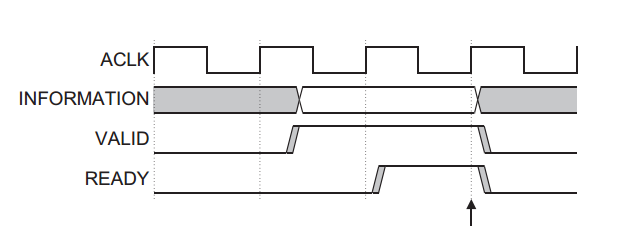
\includegraphics[width=.7\textwidth]{images/axi1handshake.png}
		\caption{Pojava \textit{VALID} pre \textit{READY}. \cite{lit4}}
		\label{fig:axi1hand}
	\end{figure}

	Na slici \ref{fig:axi1hand} se vidi da uređaj koji pruža informaciju, nakon postavljanja informacije, postavlja signal \textit{VALID} na visok logički nivo. Informacija koja je postavljena na magistralu podataka ostaje stabilna i dostupna sve dok uređaj koji treba da je primi ne postavi signal \textit{READY} na visok logički nivo, čime pokazuje da će prihvatiti informaciju koja je postavljena. Na \ref{fig:axi1hand} strelicom je prikazano kada se zapravo transfer informacije dešava. Takođe, vidi se i da se odmah nakon prosleđivanja informacije, ona uklanja.

	\begin{figure}[htb]
		\centering
		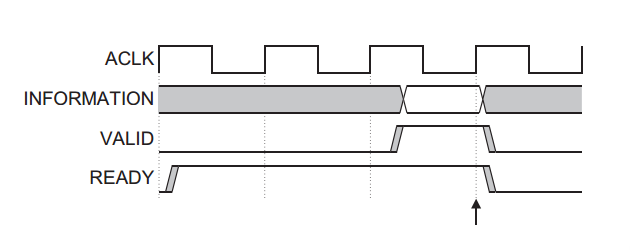
\includegraphics[width=.7\textwidth]{images/axi2handshake.png}
		\caption{Pojava \textit{READY} pre \textit{VALID} \cite{lit4}}
		\label{fig:axi2hand}
	\end{figure}

	Na slici \ref{fig:axi2hand} se vidi da uređaj koji očekuje informaciju postavlja signal \textit{READY} na logičku jedinicu i pre nego što je postavljen podatak na magistralu podataka. Ovim,  pokazuje da može prihvatiti informaciju koju je potrebno u jednom ciklusu, i to čim ona postane dostupna na magistrali. Takođe, strelica pokazuje kada se događa prenos informacije.

	\begin{figure}[htb]
		\centering
		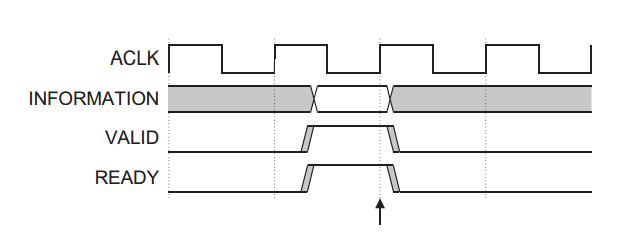
\includegraphics[width=.7\textwidth]{images/axi3handshake.png}
		\caption{Pojava \textit{READY} i \textit{VALID} istovremeno. \cite{lit4}}
		\label{fig:axi3hand}
	\end{figure}

	Na slici \ref{fig:axi3hand}, oba uređaja koja komuniciraju, istovremeno, tj. u istom ciklusu, postavljaju signale da mogu izvršiti transfer informacije. Ukoliko je to slučaj, prenos informacije se dešava momentalno. I kao i na drugim slikama, i ovde strelica pokazuje kada se zapravo događa prenos informacije od mastera do slejva, ili obrnuto. Kako su i kanali za komunikaciju odvojeni i podeljeni, tako i oni imaju svoje mehanizme rukovanja koji se razlikuju od kanala do kanala, u zavisnosti od toga kakvu funkciju oni obavljaju.

	\section{Upotreba AXI protokola u sistemu}

	Konkretno, sistem je zamišljen tako da se iskoriste prednosti ovog protokola kako bi se pokazale mogućnosti AXI u integrisanim sistemima. Periferija, odnosno uređaj koji je realizovan i nakon toga prilagođen korišćenju ovog protokola, je veoma jednostavan. Naime, ovaj uređaj obavlja neke vrlo jednostavne aritmetičke i logičke operacije, kao što su sabiranje, oduzimanje i negacija, i prosleđuje vrednosti iz jednog registra na izlaz kako bi se iskoristile mogućnosti ploče na za koju je pisana ova periferija, a to je pobuđivanje ugrađenih dioda na zc702 ploči. To je realizovano u Xilinx Vivado alatu a kod za samu periferiju je napisan u VHDL-u.

	\begin{verbatim}

	architecture Behavioral of my_periph is

	begin

    		reg0_out <= not reg0_in;
    		led_out <= reg1_in(7 downto 0);
    		reg2_out <= reg2_in + X"00000003";
    		reg3_out <= reg3_in - X"00000001";


	end Behavioral;

	\end{verbatim}

	Kako je sama periferija nedovoljna da bi se pokazale mogućnosti ovog protokola, ona je ugrađena u AXI okruženje i to konkretno AXI4-Lite za koji je napravljen samo slejv sa četiri registra koji se koriste u implementaciji ove periferije.

	\begin{figure}[htb]
		\centering
		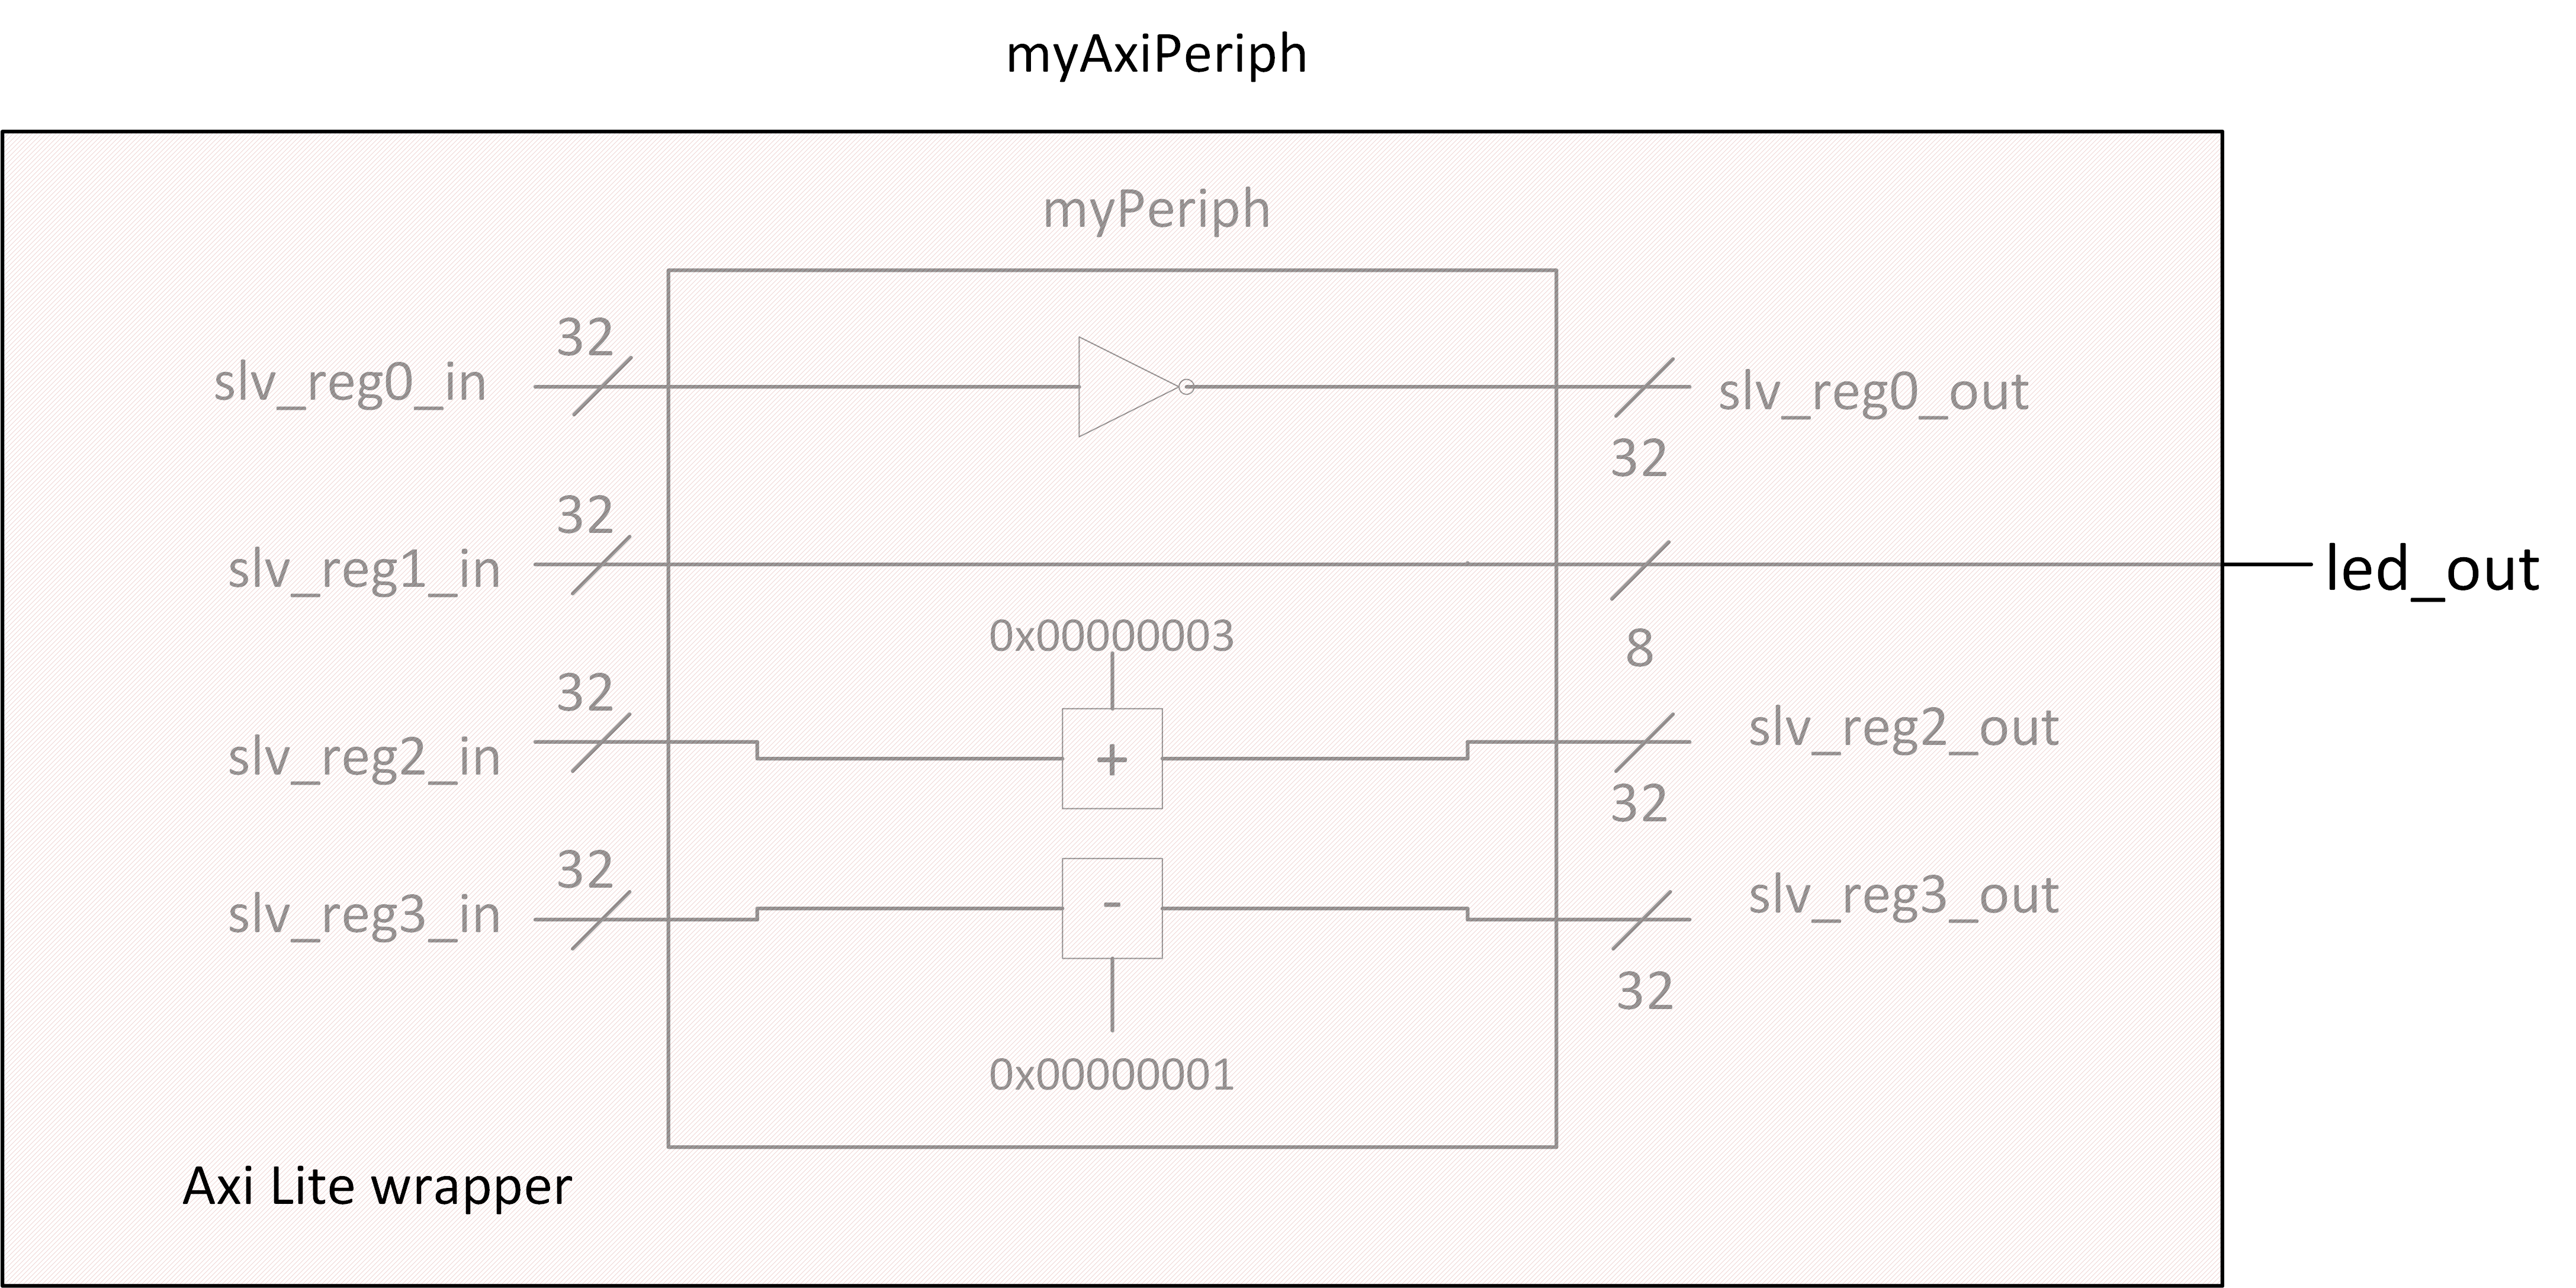
\includegraphics[width=.7\textwidth]{images/myaxiperiph.png}
		\caption{Periferija ugrađena u AXI Lite}
		\label{fig:myaxilite}
	\end{figure}

	Na slici \ref{fig:myaxilite} se vidi blok dijagram periferije koja je okružena AXI interfejsom. Kako ovaj Xilinx-ov alat generiše sam okruženje u koji se ugrađuje periferija, njegove sistemske funkcije su iskošćene za implementaciju načina pisanja i čitanja u, i iz periferije po AXI protokolu. Ova periferija je zamišljena kao primer za pristupanje nekim kontrolnim registrima određenih uređaja i čitanja statusnih registara tih uređaja.

	Vivado alat, proizvođača Xilinx, ima mogućnosti da generiše IP za hardver koji korisnik odabere. Pa tako, u ovom slučaju, izborom ploče zc702 prilikom pravljenja projekta, dobija se na uvid lista mogućnosti koje ima sam čip ZYNQ-7000 koji se nalazi na ploči. Dodavanjem ZYNQ čipa u blok dizajn projekta, moguće je konfigurisati čip prema potrebama. Na slici \ref{fig:zynqConfig} se vidi konfiguracija koja je korišćena prilikom izrade ovog sistema. Izabran je UART modul čipa kako bi testiranje bilo lakše, odnosno kako bi postojao uvid u to šta se dešava u sistemu pozivanjem jednostavnih komandi.

	\begin{figure}[h!]
		\centering
		\includegraphics[width=.63\textwidth]{images/pic4.png}
		\caption{Konfigurisanje ZYNQ čipa unutar Vivado alata}
		\label{fig:zynqConfig}
	\end{figure}

	Kako sam čip poseduje AMBA interkonekciju, dovoljno je samo dodati procesor i periferiju koja je napravljena. Periferija mora biti zapakovana kao poseban IP blok kako bi se uključila u sistem. Alat sam dodaje blok za interkonekciju, i na odgovarajući način povezuje master sa slejvom, u ovom slučaju procesor sa periferijom koja je napravljena na prikazan način. Naravno, ovaj način je moguće iskoristiti samo ukoliko se korisnik pridržava AXI protokola.	U sistemu koji je implementiran, bilo je potrebno izvesti određene pinove van samog čipa, konkretno za LE didode, pa taj deo nije mogao alat da odradi. Ovako korišćenje IP Integratora unutar Vivado alata, u mnogome omogućava jednostavno dodavanje novih delova sistema.

	\begin{figure}[htb]
		\centering
		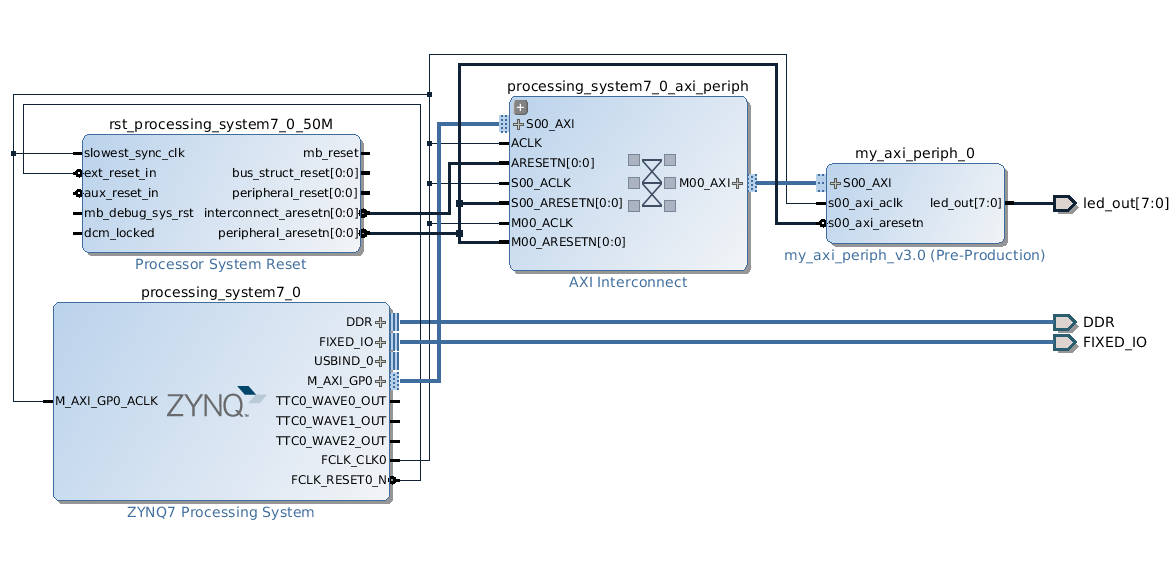
\includegraphics[width=.8\textwidth]{images/zc702system_vivado.png}
		\caption{Sistem u Vivado alatu}
		\label{fig:vivadosystem}
	\end{figure}

	Na slici \ref{fig:vivadosystem} je prikazana blok šema celog sistema. Naime, kako je već opisano od čega se sastoji ploča, i šta poseduje ZYNQ čip, ovaj alat na osnovu blok šeme sistema i uspešno odrađenih testova sinteze i implementacije, formira jedinstven VHDL wrapper, odnosno opis celog sistema u nekom HDL, u ovom slučaju VHDL. I na osnovu tog koda generiše bit fajl koji služi za programiranje stvarnog čipa na zc702 ploči.

	Testiranje digitalnog dizajna koji je napravljen je rađeno korišćenjem još jednog softverskog alata Xilinx kompanije, i to SDK (\textit{Software Development Kit}) koji je služio za programiranje mikroprocesora, koji bi koristio implementiranu periferiju u programabilnoj logici. Ovakav način proveravanja dizajna je dosta jednostavniji, i fizički prikazuje da li sistem obavalja sve što je potrebno. S obzirom da je periferija jednostavna, nije bilo potrebe za posmatranjem vremenskih dijagrama signala. Uz ovaj deo je bilo potrebno još izmeniti i ograničenja čipa, i to u smislu da se pojedini pinovi samog čipa preusmere i prikažu vrednosti određenih registara periferije, u ovom slučaju samo jednog registra koji treba da prikazuje svoj sadržaj na LE diodama na ploči. Testiranje samog dizajna se svodi na upis i čitanje iz pojednih registara, s obzirom da se prilikom izvoza sistema na mikrokontroler dobije fajl u kome su prikazane adrese memorijski mapiranih registara periferije, čijim se pristupanjem, pristupa fizičkim registrima. Kako je jedan deo testiranja bio uvid u to da li se menjaju stanja dioda na ploči, drugi deo je bio provera stanja registara unutar sistema, što je proveravano preko UART-a, odnosno čitanjem registara i prosleđivanjem na kompjuter, upoređivano je očekivano sa dobijenim, čime je zaključeno da periferija radi sve što se od nje očekuje. Ovakav način realizacije periferije prikazuje dobre osobine ovog komunikacionog protokola, a to je da je komunikacija između mastera i slejva u nekom sistemu automatizovana i vrlo jednostavna, i najvažnije da su u potpunosti razdvojeni, odnosno da postoji maksimalna sloboda u modifikovanju nekog od delova sistema, bez bojazni da će se uticati na drugi deo sistema na bilo koji način.

	\newpage

	\chapter{Linux}

	Linux je fenomen interneta. Stvoren kao hobi projekat jednog studenta, narastao do toga da je trenutno najpopularniji besplatni operativni sistem na svetu. Za mnoge ljude Linux je enigma. Kako je nešto isplativo raditi ukoliko se za to ne dobija novčana naknada? Kako u svetu u kom dominiraju velike softverske korporacije, grupa studenata ima ikakve šanse? I najvažnije, kako softver koji razvijaju različiti ljudi u različitim zemljama uopšte može da bude stabilan i efektivan? Međutim, trenutno Linux pokreće sve, od tradicionalnih personalnih kompjutera i servera pa do ugrađenih sistema (embedded systems), kao što su ruteri, pametni televizori, satelitski risiveri, i td. Takođe, najpopularniji operativni sistem na prenosivim uređajima današnjice, Android, se bazira na kernelu Linux – a.

	Koreni Linux – a se mogu naći čak i u počecima UNIX – a. 1969. godine Ken Tomson (Ken Thompson) je u Belovim laboratorijama (Bell Laboratories) eksperimentisao na operativnom sistemu sa više korisnika i operacijama sa više taskova. Uskoro mu se pridružio i Denis Riči (Dennis Richie) i zajedno su napravili početne verzije UNIX – a. Prve verzije ovog operativnog sistema su pisane u asembleru, dok je treća verzija je napisana u novom programskom jeziku. Taj novi programski jezik je C, čiji je tvorac gorepomenuti Denis Riči.

	Linux je jezgro operativnih sistema nalik UNIX-u. I trenutno u svetu postoje različite distribucije operativnih sistema koje za osnovu imaju Linux. Kernel Linux – a je osmilio i napisao Linus Torvalds 1991. godine za ličnu upotrebu, i u pročetku nije imao nikakvih namera za kros kompilacijom na druge platforme, ali se proširio i pogoni različite arhitekture, mnogo više od ostalih operativnih sistema. Kako je Linux od početka slobodan so\-ftver i softver koji se razvija putem otvorenog koda, od početka je privlačio entuzijaste koji su dosta radili na njegovom unapređenju.

	\bigskip

	Linux kernel API (\textit{Application Programming Interface}) je set interfejsa uz pomoć kojih korisnički programi komuniciraju sa kernelom, i zamišljen je da bude veoma stabilan, kako ne bi pucao u programima koji se koriste, s tim da neki programi, kao što su oni koji koriste grafički interfejs (GUI), isto tako zavise od API-a. Kao jedan deo njegove funkcionalnosti, postoje drajveri fizičkih delova sistema, odnosno hardvera, i oni koji su najpotrebniji i najstandardniji su vrlo stabilni. Međutim, interfejs između kernela sistema i modula kernela nisu smatrani za stabilne u početnom dizajnu.

	Kernel Linux – a je monolitni kernel, koji podržava pravi multi-tasking (kako u korisničkom modu, tako i, nakon 2.6. serije, u kernel modu), virtuelnu memoriju, deljene biblioteke, upravljanje memorijom, rad sa nitima, i td. Drajveri fizičkih delova sistema i dodaci kernela se pokreću u prostoru kernela, sa potpunim pristupom hardveru, sa pojedinim izuzecima koji se pokreću u korisničkom delu prostora. Grafički sistem koji velika većina ljudi koristi, se ne pokreće iz kernela, što je potpuno suprotno od onoga što se sreće kod Windows – a. Za razliku od ostalih monolitnih kernela, dodavanje i menjanje drajvera je jednostavno ukoliko se konfigurišu kao moduli kernela, i mogu se učitavati u sistem i brisati u toku izvršavanja operativnog sistema. Takođe, za razliku od standaradnih monolitnih kernela, pojedini drajveri mogu imati prednost u odnosu na druge pod određenim uslovima, što je dodato kako bi se na što bolji način rukovalo hardverskim prekidima, i da bi se dobila bolja podrška za simetrični multiprocesing, tj korišćenje više procesorskih jezgara. Hardver je takođe uključen u hijerarhiju fajlova. Pa tako programima koji upravljaju hardverom, drajverima, je moguće upravljati pristupanjem određenim fajlovima u /dev i /sys direktorijumima. Informacije o procesima su isto mapirane preko sistema fajlova, i to u /proc direktorijumu.

	\section{Programi koji upravljaju fizičkim delovima sistema, ili drajveri uređaja}

	Jedna od mnogih prednosti slobodnog operativnog sistema, je da su unutrašnji fajlovi otvoreni za pregled i modifikaciju. Operativni sistem, nekada mračno mesto koje je bilo dostupno samo malom broju programera, sada svako koga to interesuje može probati, modifikovati, učiti o tome. I sada je kernel Linux – a velika hrpa koda, do koje se mora stići na neki način, bez zahtevanja da se razume ceo kod kernela. Često, drajveri predstavljaju ulaz u svet kernela i njegovo korišćenje od strane programera.

	U narednom periodu će se samo govoriti o Linux kernelu. Drajveri imaju posebnu ulogu u kernelu. Oni su odvojene crne kutije koje čine da jedan deo hardvera odgovara na zadat način i prema zadatom interfejsu, i time sakrije kako uređaj radi. Time, korisnik dobija samo da poziva standardizovane funkcije zadatog drajvera, dok je mapiranje tih poziva na fizički uređaj posao samog drajvera. Ovaj način omogućava da se drajver razvija odvojeno od ostatka kernela, i da se nakon toga samo priključi u toku rada operativnog sistema, kad god je to potrebno. Ovakva modularnost omogućava veoma lako pisanje drajvera za Linux.

	Programeri su u mogućnosti da biraju stvari koje će uključiti u svoj dra\-jver, i u krajnjem slučaju da izaberu između vremena koje je potrebno za programiranje, i fleksibilnosti onoga što je napravljeno. Mada izgleda malo čudno da drajver može biti fleksibilan, to se odnosi na to da drajver treba da obezbedi mehanizam, a ne način korišćenja već izrađenih mehanizama. Razlika između mehanizma i politike korišćenja je jedna od najboljih ideja koja se nalazi iza dizajna UNIX – a. Većina programerskih problema se može podeliti u dva dela: „Koje mogućnosti treba omogućiti?“ – mehanizam, i „Kako se te mogućnosti mogu iskoristiti?“. Ukoliko se ova dva problema podele među različitim delovima programa, ili čak različitim programima, softverski paket koji bi trebalo time da se bavi je dosta lakši za razvoj i prilagođavanje praktičnim potrebama.

	Što se tiče drajvera, važi ista podela na mehanizam i politiku korišćenja. Na primer, DVD ili flash memorija, nemaju politiku korišćenja, zato što je njihova jedina uloga da se pokažu kao kontinualan niz blokova podataka. Viši delovi sistema pružaju politiku korišćenja, kao na primer ko sme da pristupi tim podacima, da li im se pristupa direktno ili preko sistema fajlova, i da li korisnici mogu stvoriti fajl sistem na tom medijumu. Kako različita okruženja koriste isti hardver na različite načine, potrebno je da se obezbedi da politika korišćenja ne postoji, ili da postoji u maloj meri.

	Programer koji piše drajvere bi trebalo da obrati pažnju na ovaj fundamentalni koncept, piši kernel kod za pristup fizičkom uređaju, ali nemoj nametati određenu, tebi svojstvenu, politiku korišćenja uređaja korisniku, pošto različiti korisnici imaju različite potrebe. Drajver samo treba da se pozabavi time kako da učini hardver pristupačnim za korišćenje, dok se pitanje kako koristiti hardver ostavlja primeni samog uređaja. Time drajver ostavlja dostupnost hardverskim mogućnostima bez dodavanja ikakvih ograničenja. Ponekad se ipak moraju napraviti neke odluke o politici korišćenja drajvera.

	Drajver naime predstavlja sloj softvera koji se nalazi između same primene uređaja i stvarnog hardvera. Ova privilegovana uloga koju drajver ima omogućava programeru da izabere ono što drajver treba da omogući, tako da različiti drajveri mogu stvoriti različite mogućnosti za isti hardver. U stvarnosti dizajniranje drajvera treba da predstavlja kompromis između različitih pogleda na problem koji treba da se reši drajver. Na primer, jedan uređaj može da se koristi konkurentno u različitim programima, i tu programer drajvera ima mogućnost i slobodu da obradi konkurentnost na koji god način on hoće (za koji smatra da je najbolji). Na primer, moguće je implementirati memorijsko mapiranje uređaja nezavisno od njegovih mogućnosti, ili moguće je programerima aplikativnog dela dostaviti cele biblioteke koje olakšavaju implementiranje politike korišćenja izvan već postojećih, primitivnih, i tako dalje. Najveće razmatranje koje programer u suštini ima prilikom dizajniranja drajvera je između broja opcija koje će dostaviti korisniku za zadati hardver, i vremena koje je potrebno da se dati drajver dizajnira, kao i toga da se stvari drže što jednostavnijim kako se ne bi greške provukle.

	Drajveri koji nemaju politiku korišćenja, odnosno nisu striktno vezani za jedan način korišćenja, imaju određen broj tipičnih karakteristika koje su iste za sve drajvere te vrste. Ove karakteristike uključuju podršku za sinhrone i asinhrone operacije, mogućnost da se uređaju pristupi više puta, mogućnost da se iskoriste maksimumi od datog hadvera, i manjak softverskih slojeva koji bi simplifikovali stvari ili omogućili operacije u skladu sa politikom korišćenja. Ova vrsta drajvera ne samo da bolje radi kada dođe u kontakt sa krajnjim korisnicima, već se ispostavlja da su oni lakši za stvaranje i održavanje. Ustvari, ispostavlja se da je njihovo razvijanje i cilj svih programera koji rade u ovoj oblasti.

	Međutim, većina drajvera se dostavlja sa korisničkim programima koji sami pomažu u konfiguraciji datog hardvera i komuniciranju sa istim. Ovi programi, mogu biti od jednostavnih do kompletnih grafičkih okurženja.

	\section{Delovi kernela}

	U UNIX operativnim sistemima, nekoliko konkurentnih procesa pripada različitim taskovima. Svaki proces zahteva sistemske resurse, bilo to napajanje, memorija, povezanost na mrežu, ili nešto sasvim drugo. Kernel je ustvari jedna hrpa koda koji se izvršava u funkciji upravljanja svim tim resursima. Iako razlike između različitih taskova unutar kernela nisu uvek jasno razgraničene, kernel se može podeliti na sledeće delove:

	\begin{itemize}

		\item Upravljanje procesima

	Kernel je zadužen u sistemu za stvaranje i uništavanje proesa, kao i za njihovu komunikaciju sa spoljašnjim svetom (ulaz, izlaz). Komunikacija između različitih procesa je osnova za celu funkcionalnost sistema i isto je za to zadužen kernel. Kao dodatak svemu tome, kernel poseduje i jedan raspoređivač (\textit{the scheduler}), koji kontroliše kako konkurentni procesi u krajnjem slučaju koriste CPU. Uopšteno, deo kernela koji se bavi upravljanjem procesima, implementira nekolicinu procesa na jednom ili više procesora, zavisno od sistema koji se koristi.

		\item Upravljanje memorijom

	Memorija je najbitniji resurs u jednom sistemu, i politika njenog korišćenja može biti od kritične važnosti za performanse sistema. Kernel prilikom pokretanja stvara virtuelni adresni prostor za sve procese na ograničenim resursima. Različiti delovi kernela komuniciraju sa podsistemom za memoriju preko određenog broja funkcija, čiji je raspon od jednostavnih malloc/free funkcija do mnogo kompleksnijih.

		\item Sistemi fajlova

	Unix je baziran na konceptu sistema fajlova. Sve unutar UNIX – a se može tretirati kao fajl. Pa tako kernel prilikom pokretanja pravi struktuirani sistem koji upravlja fajlovima, i to nad nestruktuiranom hardveru, čija se apstrakcija fajlova kasnije koristi kroz ceo sistem. Kao dodatak, Linux podržava dosta tipova fajl sistema, i to kao način ogranizovanja podataka na jednom fizičkom medijumu.

		\item Kontrola uređaja

	Skoro svaka sistemska operacija eventualno se mapira za fizički uređaj. Sa izuzetkom procesora, memorije i nekoliko drugih, sva ostala kontrola hardvera se obavlja preko posebnog koda koji je poseban za uređaj koji je adresiran. Ovaj kod se naziva drajver uređaja. U kernel mora biti ugrađen drajver za svaku periferiju koja se koristi u sistemu, od hard diska do tastature.

		\item Komunikacija

	Komunikacija između ostalih sistema, kako lokalna tako i globalna povezanost se mora upravljati uz pomoć operativnog sistema, zato što većina komunikacionih operacija nije specificirana za određen proces, s obzirom da su paketi informacija asihrono stižu. Ti paketi se moraju skupiti, identifikovati, i rastaviti pre nego što pređu na obradu podataka koji su pristigli. Sistem je zadužen za dostavljanje paketa kroz programe i interfejse komunikacije, i mora se kontrolisati pokretanje programa na osnovu njegove aktivnosti u komuniciranju.

	\end{itemize}

	\section{Moduli kernela}

	Jedna od dobrih mogućnosti Linux – a je mogućnost proširenja seta funkcija koji postoji u kernelu. Ovo znači da se različite funkcionalnosti mogu dodavati i uklanjati iz kernela dok sistem radi. Bilo koji deo koda koji je moguće dodati u kernel u toku izvršavanja se naziva modul kernela. Kernel Linux – a podržava nekoliko različitih tipova, ili klasa, modula, uključujući i drajvere uređaja. Svaki modul se stvara iz objektnog koda (nije napravljen kompletan fajl koji se može izvršavati), koji se može dinamički linkovati u kernel koji već radi i to uz pomoć insmod() funkcije, kao i izbrisati iz kernela uz pomoć rmmod() funkcije.

	\begin{figure}[htb]
		\centering
		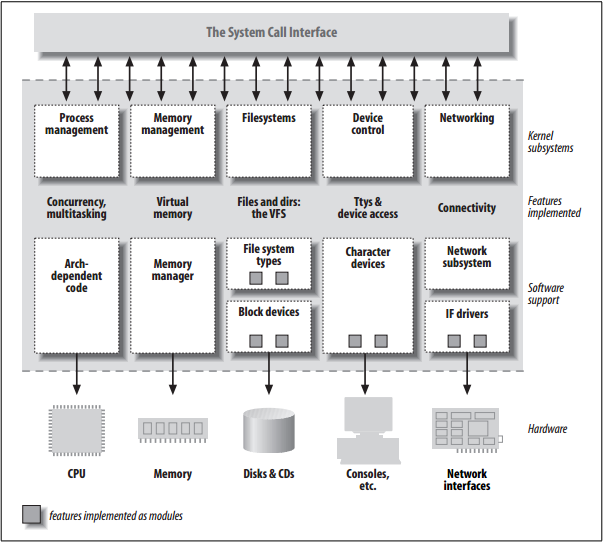
\includegraphics[width=.8\textwidth]{images/kernelsplit.png}
		\caption{Kernel moduli}
		\label{fig:kernelmodul}
	\end{figure}

	Slika \ref{fig:kernelmodul} prikazuje različite klase modula koji mogu obavljati neke specifične zadatke – kaže se da modul pripada određenoj klasi samo na osnovu funkcionalnosti koje pruža. Raspored modula na slici pokriva najbitnije klase, ali nije ni blizu kompletne slike modula, jer se sve više funkcionalnosti Linux – a modularizuje.

	\section{Klase uređaja i modula}

	Način na koji Linux razdvaja sve uređaje se u osnovi deli na tri osnovna tipa. Pojedinačni moduli obično implementiraju jedan od ovih tipova, i u osnovi klasifikacija se svodi na char module, block module i network module. Podela modula u druge tipove, ili klase, nije baš striktna, na primer programer može napraviti veliki modul koji će implementirati različite drajvere u jednoj velikoj šumi koda. Ali ipak, dobar način programiranja zahteva da se stvaraju različiti moduli za svaku novu funkcionalnost koju implementiraju, zato što je dekompozicija ključni elemnt skalabilnosti i modularnosti.

	Ove tri klase su:

	\begin{itemize}

		\item \textit{Character devices}

	Ovaj tip uređaja je takav da mu se može pristupti kao nizu bajtova, kao fajlu, i drajver za ovaj tip uređaja služi da implementira ovakav način ponašanja. U osnovnom slučaju, drajver implentira samo funkcije koje služe za otvaranje fajla, zatvaranje, upis i čitanje. Tekstualna konzola (/dev/console) i serijski port (/dev/ttyS0 i ostali) su primeri ovih uređaja, kako su dobro prikazani na osnovu niza bajtova, odnosno podataka. Char uređajima se pristupa preko čvorova, odnosno fajlova u fajl sistemima, kao što su /dev/tty1 i /dev/lp0. Jedina bitna razlika između fajlova koji predstavljaju char uređaje i običnih fajlova je u tome da se u običnim fajlovima korisnik može kretati napred i nazad unutar fajla, dok su fajlovi koji predstavljaju uređaji kao kanali podataka, kojima se pristupa sekvencionalno. Postoje, naravno i uređaji koji su slični prostoru podataka, gde se korisnik može kretati kako on hoće.

		\item \textit{Block devices}

	Kao i prethodna grupa uređaja, block uređajima se pristupa preko fajlova fajl sistema u /dev folderu. Ovaj tip uređaja su oni uređaji na kojima se može stvoriti fajlsistem. U većini UNIX sistema, ovi uređaji samo mogu obavljati operacije ulaza i izlaza, odnosno prenositi jedan ili više blokova memorije, koji su obično dužine 512 bajtova. Dok Linux dozvoljava aplikacijama čitanje i pisanje u block uređaje isto kao i u char uređaje. Kao rezultat ovoga, razlika ova dva tipa uređaja se svodi samo na to kako kernel njima interno upravlja, i na osnovu toga u kernel – drajver interfejsu. Kao i char, block tipu uređaja se pristupa preko fajla u fajlsistemu.

		\pagebreak

		\item \textit{Network interfaces}

	Sav prenos podataka se obavlja kroz interfejs, tj kroz uređaj koji omogućava komunikaciju sa ostalim uređajima. Tipično, interfejs je neki fizički uređaj, mada može biti i čisto softverski uređaj, odnosno neki program. Interfejs za komunikaciju je zadužen za slanje i primanje paketa podataka koji se pokreće na osnovu dela kernela koji je zadužen za komunikaciju, a da nema uvid u to koliko je ustvari veliko to što se prenosi. Većina mrežnih konekcija su orijentisane na tok podataka, ali su uređaji koji služe za povezivanje, tipično dizajnirani samo za prijem i predaju paketa podataka. Drajver koji pogoni mrežni uređaj ne zna ništa o karakteristikama konekcije, već samo vodi računa o upravljanju paketima.

	\end{itemize}

	Naravno, postoje i druge klasifikacije drajver modula koje su ortogonalne ovoj koja je navedena. Uopšteno, neki tipovi drajvera rade i sa dodatnim slojevima kernel podrške za dati tip uređaja.

	\section{Razlike između kernel modula i aplikacija}

	Dok male i srednje aplikacije obave samo jedan zadatak od početka do kraja, svaki kernel modul se registruje kako bi služio budućim pozivima, i njegova funkcija koja ga inicijalizuje se završava odmah. Drugim rečima inicijalizaciona funkcija je tu da pripremi kasnije pozive unutrašnjih funkcija pojedinačnih modula. Funkcija kraja jednog modula se poziva kada se modul gasi, i označava kraj dostupnosti modula za naredne pozive. Ovakav pristup programiranju je veoma sličan programiranju koje se zasniva na događajima. Dok aplikacije nisu bazirane na događajima, svi kernel moduli jesu. Druga bitna razlika između aplikacija koje su bazirane na događajima, i kernel koda je u funkciji napuštanja, tj. dok aplikacije mogu biti lenje i sa zakašnjenjem oslobađati alocirane resurse ili čak uopšte ne osloboditi neke resurse, kernel funkcija mora pažljivo uništiti sve što je funkcija za inicijalizaciju napravila, ili će delovi ostati dok se sistem ne resetuje.

	Aplikacije obično počinju funkcijom main(), koja izvrši gomilu instru\-kci\-ja, i aplikacija se završi kada se završi izvršavanje tih instrukcija. Međutim kernel moduli rade na drugi način. Modul uvek počinje funkcijom init\_module ili funkcijom koju je sam programer definisao  pozivom module\_init. Ovo je funkcija kojom započinje rad jednog modula, i govori kernelu da su omogućene funkcionalnosti koje modul ima i postavlja modul na korišćenje kernelu. Ova funkcija se izvrši jednom, i nakon toga modul ne radi ništa sve dok kernel ne odluči da iskoristi funkcionalnosti koje pruža taj kernel modul. Svaki modul mora posedovati funkciju koja stavlja modul u stanje pripravnosti, kao i funkciju koja ukida taj modul iz konteksta kernela.

	Programeri svakodnevno koriste funkcije koje oni ne definišu, kao na primer printf(). Tj. koriste funkcije koje se nalaze u standardnoj biblioteci C jezika. Definicije ovih funkcija se ne ubacuju u program sve do faze linkovanja, koja osigurava da kod za određenu funkciju koja je pozvana bude dostupan, i popravlja poziv funkcije koji ukazuje baš na kod koji je potreban.

	Ovde su kernel moduli dosta drugačiji. Na primer, umesto standardne funkcije u jeziku C printf(), u kernelu se koristi funkcija printk(), ali za njeno korišćenje nije potrebno uključiti standardnu biblioteku unutar koda gde se koristi. Naime, kernel moduli su objektni fajlovi čiji se simboli određuju prilikom instanciranja modula. Gde definicija simbola dolazi direktno od kernela, i jedine funkcije koje se mogu eksterno koristiti su one koje kernel obezbedi.

	To je jedna od razlika između standardnih aplikacija i kernel modula. Međutim bibliotečke funkcije su funkcije višeg nivoa, one se pokreću kompletno u korisničkom režimu i pružaju mnogo prijatniji interfejs programeru ka funkcijama koje rade stvaran posao – sistemskim pozivima. Naime, sistemski pozivi su pozivi funkcija koje se pokreću u kernel režimu za korisničke aplikacije i obezbeđuje ih kernel. Standardna funkcija printf() možda izgleda kao opšta funkcija za prikazivanje, dok ona samo formatira određenu nisku znakova na način koji je korisnik odabrao, i prosleđuje je sistemskom pozivu nižeg nivoa write(), koja šalje taj tekst na standardni izlaz.

	\section{User space vs. Kernel space}

	Kernel je sav napravljen i postoji samo zbog upravljanja i pristupa resursima, bilo da je resurs grafička kartica, hard disk, ili memorija. Programi se obično nadmeću kako bi dobili iste resurse. Tu na scenu stupa kernel, on je tu kako bi se stvari odvijale u nekom redu, i kako ne bi omogućio korisnicima pristup resursima kad god oni to hoće, već kada je to bezbedno za ceo sistem.

	Dok se aplikacija pokreće u korisničkom prostoru, modul se pokreće u kernel prostoru. Ovaj koncept je u osnovi teorije operativnih sistema. Uloga operativnog sistema, u praksi, ja da obezbedi programima kozisentan pristup hardveru kompjutera. Dodatno, operativni sistem mora obezbediti nezavisne operacije u programima i zaštititi ih od nedozvoljenog pristupa resursima. Ovaj netrivijalan zadatak je jedino moguć ukoliko CPU zahteva zaštitu sistemskog softvera od aplikacija. Svaki procesor novijih generacija može da obezbedi ovu mogućnost. Ovakav izbor pristupa je kako bi se implementirali različiti operativni modaliteti ili nivoi u samom CPU. Ovi nivoi imaju različite uloge, i neke operacije su zabranjene na nižim levelima, pri čemu programski kod može prelaziti sa jednog na drugi nivo samo preko ograničenog broja kapija (gates). UNIX sistemi su dizajnirani tako da koriste prednosti ove hardverske mogućnosti, i to koristeći dva ovakva nivoa. Svi sadašnji procesori imaju minimum dva nivoa, dok neki imaju i više. Ukoliko postoji više od dva ovakva nivoa, koriste se najviši i najniži. U UNIX – u, kernel se pokreće na najvišem nivou (mod supervizora), gde je sve dozvoljeno, dok se aplikacije pokreću na najnižem nivou (mod korisnika), gde procesor reguliše direktan pristup hardveru i nedozvoljen pristup memoriji.

	Obično se ovi režimi pominju samo kao kernel prostor i korisnički prostor (\textit{kernel space and user space}). Ovi termini ne obuhvataju samo različite nivoe privilegija koje proističu iz ova dva režima, već i činjenica da svaki režim može imati svoju mapiranu memoriju, i svoj adresni prostor takođe.

	UNIX prebacuje pokretanje iz korisničkog ka kernel režimu kad god aplikacija izda sistemski poziv ili kada je prekinuta preko hardverskog prekida. Kernel kod koji izvršava sistemske pozive radi u kontekstu procesa, tj radi u ime procesa koji se poziva i koji može da pristupi podacima u adresnom prostoru datog procesa. Kod koji rukovodi prekidima, na drugoj strani, je asinhron u odnosu na procese i nije povezan ni sa jednim konkretnim procesom.

	Uloga modula je da proširi funkcionalnost kernela, odnosno modularan kod se pokreće u kernel režimu. Obično platforma drajvera obavlja zadatke koju su već pomenuti. Neke funkcije u modulu se izvode u okviru sistemskih poziva, a neki su zaduženi za rukovanje prekidima.

	\section{Konkurentnost u kernelu}

	Jedan od razloga zašto je kernel programiranje toliko različito od konvencionalnog programiranja aplikacija je konkurentnost. Većina aplikacija, sa izuzetkom višenitnih aplikacija, se izvršava sekvencijalno, od početka do kraja, bez bojazni da će nešto u toku izvršavanja promeniti okruženje. Svet kernel koda nije tako jednostavan, čak i najmanji kernel modul se mora dizajnirati tako da se dosta stvari može desiti odjednom.

	U modernim Linux sistemima, postoji nekoliko izvora konkurentnosti, i u skladu sa tim postoji opasnost od utrkivanja. Utrkivanje predstavalja problem koji nastaje kada izlaz nekog sistema, softverskog ili hardverskog, zavisi od sekvence događaja ili vremena nekih drugih nekontrolisanih sistema. To postaje problem po sistem kada se događaji ne dese u redu koji je programer predvideo. Ideja utrkivanja potiče od zamisli dva signala koji se utrkuju koji će pre izazvati promenu na izlazu. Naime, više procesa koji se vrte u korisničkom režimu mogu izvršavati napisan kod u mnogo različitih scenarija. Simetrični multiprocesorski sistemi mogu čak izvršavati napisan kod na različitim prcesorima, a kamoli u različitim kontekstima.  Kernel kod zavisi od konteksta u kome se nalaze svi procesi, tj. onaj proces koji je većeg prioriteta, izvršava kod, pre onoga koji ima manji prioritet. Shodno tome, drajver koji je napisan može izgubiti procesor u bilo kom trenutku. Čak i proces koji ga nasledi može koristiti isti kernel kod, koji će pokretati isti uređaj.

	Prirodno, Linux sistemi pokreću nekoliko procesa, sigurno više od jednog koji će probati da koriste implementiran drajver u isto vreme. Većina uređaja ima mogućnosti da prekine procesor, prekid se obraćuje asinhrono i može se pozvati u isto vreme kada drajver pokušava da uradi nešto drugo. Takođe, Linux se može koristiti na multiprocesorskim sistemima, tako da drajver može izvršavati konkurentnost na više od jednog CPU – a. Odatle, kernel kod mora biti otporan, odnosno mora biti sposoban da se pokreće u više od jednog konteksta u isto vreme. Strukture podataka se moraju pažljivo praviti tako da zadrže odvojeno izvršavanje više niti, i kod mora voditi računa o pristupu deljenih podataka tako da spreči podatke da postanu neupotrebljivi. Dobro upravljanje konkurentnosti je potrebno kako bi se napisao ispravan kernel kod, i iz tog razloga čak i jednostavni drajveri se moraju pisati u skladu sa principom konkurentnosti.

	\section{File systems}

	Kao što je već navedeno kernel Linux – a ima dve primarne funkcije, a to su da kontroliše pristup fizičkim uređajima koji su deo kompjuterskog sistema, i da raspoređuje kad i kako koji proces koristi te uređaje. Folder /proc/, poznatiji kao proc fajl sistem sadrži hijerarhijski složene specijalne fajlove koji predstavljaju trenutno stanje kernela sistema, i takođe dozvoljava programima i korisnicima da pristupe pogledu kernela na sistem. Unutar ovog direktorijuma mogu se naći informacije koje opisuju ceo hardverski deo sistema i sve procese koji se trenutno odvijaju u sitemu. I dodatno, postoje neki fajlovi kojima mogu upravljati korisnici, putem aplikacije ili lično kako bi napravili neke konfiguracione promene u kernelu.

	U Linux – u je sve fajl, i svi podaci koji se nalaze na sistemu se nalaze u fajlovima, bilo binarnim, bilo tekstualnim. Međutim, unutar /proc/ foldera se nalaze fajlovi drugog tipa, koji se često naziva virtualnim tipom fajla. Pošto se ovaj fajl sistem često pominje u kontekstu virtuelnog fajl sistema. Naime, ovi virtuelni fajlovi poseduju jedinstvene kvalitete. Većina njih zauzima 0 bajtova, a ipak sadrže gomilu informacija kada se otvore. Kao i dodatno, većina podešavanja za vreme i datum se odnose na trenutne informacije o vremenu, što se odnosi na to da se konstantno osvežavaju. Neki od ovih fajlova sadrže informacije o sistemskom hardveru i uvek su u toku sa stanjem hardvera, dok drugi sadže konfiguracione informacije i interfejse prema drugim uređajima.

	\newpage

	\chapter{Softverska realizacija}
	Ploča na kojoj je sistem razvijan, ZC702 firme Xilinx, poseduje interfejs koji omogućava korisnički pristup opšte namene za SDIO nepromenjive memorijske kartice i periferije. Kako ovo razvojno okruženje poseduje mogućnost inicijalizacije sistema na nekoliko načina, inicijalizacija pomoću memorijske kartice je veoma jednostavna, i pogodna za pokretanje Linux operativnog sistema na samoj ploči. Kao što je već navedeno Linux sistem je pogodan za primenu u ugrađenim sistemima, pa je u razvoju ovog sistema bilo logično koristiti njegove pogodnosti. Kako bi se operativni sistem koristio na ovoj ploči, potrebno je pripremiti samu ploču, ali i medijum na kome će se nalaziti sam sistem koji treba pokrenuti. Memorijska kartica je u ovom slučaju napravljena tako da nakon uključenja napajanja ploče pokreće određene fajlove koji dovode do podizanja sistema. Naravno, promenom stanja određenih prekidača na samoj ploči određuje se način inicijalizacije. Medijum koji je korišćen je podeljen na particije tako da jedan deo kartice predstavlja deo na kome će se nalaziti fajlovi neophodni za podizanje sistema (\textit{BOOT}), dok je drugi deo kartice fajl sistem na kome će se nalaziti ceo operativni sistem kada se podigne (\textit{ROOT}). Način na koji su napravljene particije, kao i formati samih particija su u skladu sa uputstvima proizvođača ploče kako bi se postigao zahtevani rezultat.

	Priprema samih fajlova je odrađena takođe u skladu sa preporukama proizvođača ploče koja je korišćena. S tim u vezi, napravljena je Linux \textit{shell} skripta, prikazana u celosti unutar dodatka \ref{a:compile}, koja će izvršavati celokupan postupak kako bi se dobili određeni fajlovi koji su potrebni za pokretanje Linux-a sa memorijske kartice. Proizvođač je naveo i koje je verzije kernela i alata za kros kompilaciju potrebno koristiti, kao i linkove odakle je moguće skinuti sve što je potrebno.

	\pagebreak

	Kros kompilacija predstavlja proces kompilacije određenog koda za arhitekturu za koju se pravi sam kod, odnosno gde će se koristiti. Svi potrebni alati se nalaze na git adresama Xilinx-a, koje su navedene u literaturi.

	Pre nego se krene sa izvršavanjem koraka koji su prikazani na slici \ref{fig:flow}, potrebno je da se uveze alat koji je već korišćen, Xilinx SDK, kako bi se iskoristile njegove već postojeće mogućnosti, kao i definisati tip kros kompajlera koji se koristi, odnosno arhitekturu za koju se kompajlira kod.

	\begin{figure}[htb]
		\centering
		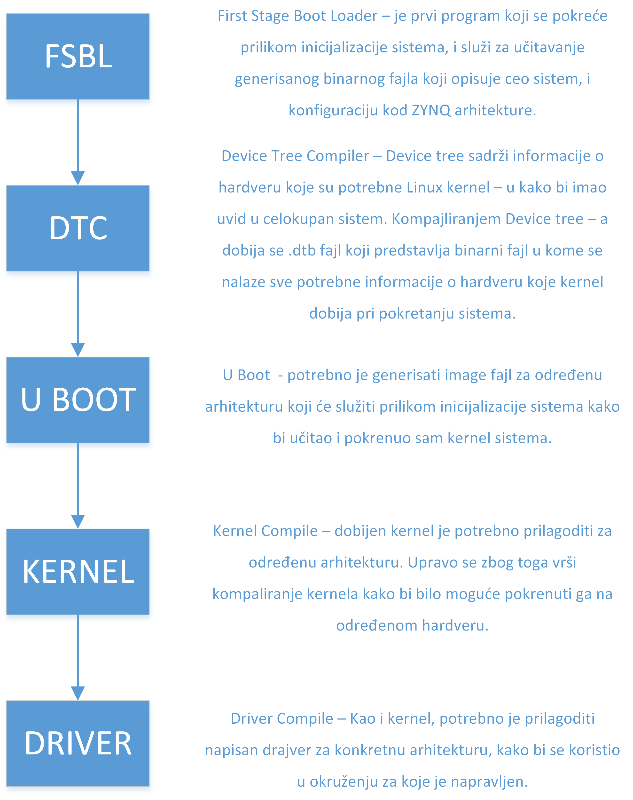
\includegraphics[width=.8\textwidth]{images/flowCompile.png}
		\caption{Dijagram toka kompilacije potrebnih fajlova za pokretanje Linux-a na ploči}
		\label{fig:flow}
	\end{figure}

	Na slici \ref{fig:flow} su prikazani koraci koje je potrebno proći na zadati način kako bi se dobio set fajlova koji su potrebni za ispravnu inicijalizaciju sistema na samoj ploči. Na slici su takođe prikazani i principski opisi koraka koji se izvršavaju. Na osnovu svih izgenerisanih fajlova, prilikom pokretanja ploče sa ovim fajlovima dobija se čist Linux sistem na ploči koji je moguće koristiti. Uvid u to šta se dešava na samoj ploči se dobija povezivanjem na serijski terminal ploče, preko koga se dobijaju svi potrebni podaci na korisničkom kompjuteru. Takođe, sve komande koje se pozivaju za sistem na ploči se šalju serijski preko UART – a. Ovim postupcima je dobijen kompletno funkcionalan operativan sistem koji se pokreće na hardveru koji predstavlja kompletan kompjuterski sistem, i koji se može prilagoditi korisničkim potrebama.

	\section{Linux modul}
	Uređaj za koji se pravi drajver je posmatran kao \textit{CHAR} uređaj zato što ovaj tip uređaja predstavlja jednostavne uređaje, što je ovde u pitanju. Ovom tipu uređaja se pristupa preko imena u fajl sistemima. Ova imena se nazivaju i specijalnim fajlovima, fajlovima uređaja, ili jednostavno čvorovima u strukturi fajl sistema (fajl sistem, folder organizovan kao binarno stablo), i oni se čuvaju u /dev folderu. Ove fajlove, tj fajlove koji predstavljaju \textit{CHAR} uređaje prepoznajemo po početnom slovu C prilikom pozivanja terminalne komande ls -l unutar /dev foldera. Takođe \textit{BLOCK} uređaji se pojavljuju u istom folderu, samo se oni prepoznaju po početnom slovu B. Prilikom pozivanja pomenute komande ls -l primećuju se brojevi pored opisa fajla unutar pomenutog foldera. Ovi brojevi se prestavljaju kao Glavni i Sporedni broj (\textit{major and minor number}), pri čemu glavni broj određuje koji drajver se koristi kako bi upravljao zadatim hardverskim delom, dok se sporedni broj koristi kako bi kernel mogao da odredi tačno koji uređaj se koristi u tom trenutku, odnosno koji uređaj poziva drajver.

	\begin{figure}[h!]
		\centering
		\includegraphics[width=.7\textwidth]{images/pic1.png}
		\caption{Prikaz rezultata poziva funkcije \textit{ls -l} na ploči unutar direktorijuma \textit{dev}}
		\label{fig:lsl}
	\end{figure}

	\bigskip

	Prilikom implementacije ovog drajvera, ostavljeno je kernelu da sam dinamički odredi potrebne brojeve. Unutar kernela, postoje vrlo bitne strukture podataka, koje predstavljaju file\_operations, file, i inode.

	\begin{itemize}

		\item \textit{file\_operations}

	Sami brojevi, Glavni i Sporedni, označavaju da je uređaj u kontekstu kernela, i da kernel ima svest o njemu. Međutim, potrebno je dodati neke funkcije tim brojevima, odnosno omogućiti da se prilikom obraćanja tim brojevima nešto promeni. A to može jedino ukoliko strukturi file\_operations dodelimo neke funkcije, koje će se pokretati kada kernel uspostavi komunikaciju sa drajverom, odnosno uređajem. Ova strukutra ustvari predstavlja kolekciju pokazivača na funkcije. Svaki otvoren fajl (koji je predstavljen strukturom file), je povezan sa sopstvenim setom funkcija. Operacije koje se odvijaju nad modulima su u osnovi jednostavne, otvranje fajla, čitanje iz njega, pisanje, i td. Ovo razmišljanje dovodi do toga da fajl predstavljamo kao objekat, a funkcije kao metode, koristeći objektno – orjentisanu terminologiju. Što je mnogo jednostavnije za razvijanje i korišćenje. Svaki deo strukture file\_operations mora predstavljati pokazivač na funkciju koja implementira neku funkcionalnost drajvera, ili postaviti taj deo na vrednost NULL, čime se označava da ta funkcionalnost nije podržana. Konkretno, za razvijanje ovog drajvera su implementirane samo osnovne funkcije, i to read, write, open, llseak, release, koje će biti opisane u kasnijem tekstu.

		\bigskip

		\item \textit{file}

	Struktura file je druga najznačajnija struktura koja se koristi u drajverima uređaja. I ona se veoma razlikuje od standardne FILE strukture koja je definisana u C standarnoj biblioteci. Ova struktura unutar kernela predstavlja otvoren fajl, nije specifično samo za drajvere, svaki fajl unutar sistema ima dodeljenu strukturu FILE unutar kernel okruženja. Ova struktura se stvara prilikom pozivanja funkcije za otvaranje fajla drajvera, i prosleđuje se onoj funkciji koja zahteva operisanje nad tim fajlom, sve dok se ne zatvori sam fajl i uređaj skloni iz liste dostupnih. Nakon što se zatvore sve instance jednog fajla, kernel dealocira potrebnu memoriju koju je koristio konkretan fajl, i vrati sve resurse koje je koristio.

		\bigskip

		\item \textit{inode}

		Ovu strukturu kernel koristi kako bi interno predstavio fajlove. Pa je stoga različita u odnosu na prethodnu strukturu koja predstavlja deskriptor otvorenog fajla. Naime može postojati nekolicina file struktura koje predstavljaju jedan uređaj u različitim scenarijima, ali sve te strukture ukazuju na samo jednu inode strukturu. I ova struktura poseduje veliku količinu informacija za konkretan fajl.

	\end{itemize}

	Kao što je prethodno navedeno, /proc fajl sistem je poseban, softverski kreiran fajl sistem koji je korišćen od strane kernela da eksportuje informacije ka spoljašnjem sistemu. Svaki fajl unutar /proc direktorijuma je vezan za kernel funkciju koja generiše sadržaj fajla u trenutku kada se pokuša čitanje konkretnog fajla. Ovaj fajl sistem se mnogo koristi u Linux – u, jer većina drajvera eksportuje informacije preko ovog fajl sistema, kao što je napravljeno i u sistemu koji je predmet ovog rada. Svi moduli koji rade sa ovim fajl sistemom, pa i ovaj koji se ovde pominje, moraju uključiti u svoj kod <linux/proc\_fs> biblioteku kako bi određene funkcije bile definisane. U ovom slučaju sve funkcije koje su potrebne za upravljanje fajlom, a tim i hardverom za koji je vezan ovaj kod, moraju se definisati tako da odgovaraju potrebama konkretnog uređaja. U sklopu ovih funkcija moraju biti i funkcije koje će stvarati podatke kada se pokuša čitanje datih fajlova, kao što je i pomenuto prethodno. Kada proces pokuša čitanje iz /proc fajla koji predstavlja uređaj, kernel alocira jednu stranicu memorije podrazumevane veličine, gde drajver može da postavlja podatke koji će se videti u korisničkom prostoru. I potrebno je da programer predefiniše funkcije za čitanje i pisanje u taj određen fajl, kako bi hardver imao uvid u to šta se dešava u korisničkom prostoru.

	Kako je bilo potrebno da se implementirani sistem uključi u operativni sistem, određene funkcije je bilo potrebno definisati tako da omoguće komunikaciju između kernel prostora i korisničkog prostora. Kao što je već navedeno, ovaj sistem je veoma jednostavan, četiri registra nad kojima se obavljaju neke operacije. Ovaj sistem je moguće posmatrati i kao deo većeg sistema, pri čemu su ovi registri, statusni registar, kontrolni registar, i tako dalje, u nekom ugrađenom sistemu, za koji je potrebno omogućiti da se pročita njihov sadržaj i upiše novi. Na osnovu toga, bilo je potrebno implementirati funkcije koje se odnose upravo na to, funkcije za otvaranje fajla, štampanje vrednosti registara, pisanje u registre, i td.

	Kao što je i navedeno, funkcije su takve da implementiraju korišćenje svih prethodno pomenutih mogućnosti i struktura ovog fajl sistema. Pa tako, funkcija koja samo služi za otvaranje fajla prima \textit{INODE} i \textit{FILE} parametre i alocira određen memorijski prostor koji će služiti za smeštanje podataka u taj fajl. Funkcija za štampanje registara samo poziva sistemsku funkciju za čitanje sa određene adrese ioread32(), koja predstavlja trenutnu adresu u tom ciklusu korišćenja fajla unutar fajl sistema.

	Telo funkcije za prikaz vrednosti sa trenutne adrese:

\begin{verbatim}
myValuePrint = ioread32(addr);  //current virtual address
seq_printf(file, "0x%x \n", myValuePrint);
return 0;
\end{verbatim}

	Najbitnija funkcija u ovom drajveru je funkcija pisanja u fajl, i to zato što je potrebno pristupiti registru u memoriji po izboru. Zaglavlje funkcije za pisanje u fajl unutar /proc fajl sistema:

\begin{verbatim}

static ssize_t proc_my_write (struct file *file,
const char __user *buf, size_t count, loff_t *ppos)

\end{verbatim}


	Kako se prilikom poziva funkcije za upis u fajl prosleđuje cela niska znakova koja sledi za ključnom rečju funkcije, potrebno je prepoznati kad se šalje ofset od bazne adrese, a kad se prosleđuje podatak. Tu je iskorišćena sloboda programera da sam odluči šta se kad prosleđuje, pa je u ovom slučaju uvedena konvencija da se prvo šalje ofset koji se predstavlja kao broj registra kome se pokušava pristupiti, dok je drugi podatak koji stiže podatak koji se želi upisati u taj registar. Što je i implementirano. Međutim, kako je potrebno napraviti i način da se čita iz registra po želji, onda je potrebno opet koristiti funkciju za upis kako bi se promenila trenutna adresa na koju će odvesti upis u taj fajl. U ovom slučaju to je napravljeno uz pomoć ograničenja ofseta, tj. ukoliko korisnički prostor pošalje drajveru broj registra koji prelazi broj registara koji poseduje uređaj, onda se radi o pokušaju čitanja iz uređaja, i nakon toga drajver ne očekuje podatak, dok ukoliko broj registra upada u opseg registara, onda se očekuje i podatak za upisivanje. Programski kod koji implementira ove funkcionalnosti je dat u okviru dodatka \ref{a:driver}. Za prenos podataka iz korisničkog u kernel prostor su korišćene fabričke funkcije koje se nalaze u kernelu. I to za ovaj slučaj konkretno funkciju copy\_form\_user() koja se nalazi kao deo standardne biblioteke <asm/uaccess.h>. Ostale funkcije koje su potrebne kako bi struktura file\_operations bila kompletna, read, llseek, release, korišćene su sistemske funkcije seq\_read, seq\_lseek, single\_release, koje se nalaze u biblioteci <linux/seq\_file.h>. Pri čemu funkcija llseek() predstavlja metod koji se koristi kako bi promenio trenutnu poziciju za pisanje, odnosno čitanje, unutar fajla, gde se trenutna pozicija dobija kao povratna vrednost funkcije koja je tipa loff\_t koja je minimum 64 bitna veličina, čak i na 32 bitnim arhitekturama. Funkcija read() se poziva kada se pokušava čitanje iz fajla. Dok je funkcija release() pozvana kada se oslobađa fajl struktura. Dve poslednje funkcije mogu biti NULL, međutim ovde su uzete sistemske funkcije seq\_file biblioteke.

	Prikaz stukture file\_operations koja je implementirana, gde su pojedinačne funkcije prikazane u dodatku \ref{a:driver}:

\begin{verbatim}
static const struct file_operations procMyOperations =
{
    .open = proc_my_open,
    .read = seq_read,          //default function from seq_file
    .write = proc_my_write,
    .llseek = seq_lseek,       //default function from seq_file
    .release = single_release  //default function
};
\end{verbatim}

	Kako je već objašnjeno, svaki drajver, odnosno deo koda koji opisuje neki uređaj, mora imati neku pristupnu tačku. Odnosno, moraju se definisati Glavni i Sporedni broj, kako je gore pomenuto, i povezati konkretne brojeve sa hardverom. Isto kao prethodno, ovaj deo je u velikoj meri automatizovan, pa postoji struktura platform\_driver uz pomoć koje se automatski dobija standardni model drajvera, za koji je već urađena enumeracija. Programeru se ostavlja da sam implementira funkcije koje služe za inicijalizaciju uređaja i njegovo brisanje iz kernela. Ovo se postiže implementacijama metoda probe() i remove(), unutar kojih je potrebno alocirati memoriju kernela koju će koristiti uređaj, kreirati sam ulaz kroz /proc fajl sistem, i vratiti informaciju o tome. Takođe metoda remove() služi da „pospremi“ sve što je u nekom trenutku napravljeno. Ove dve metode se mogu posmatrati kao metode inicijalizacije i brisanja kernel modula iz sistema. Ono što je veoma bitno za korišćenje ovih struktura jeste povezivanje sa konkretnim hardverom, tj hardverom koji je opisan unutar kernelovih fajlova koji prikazuju šta je uključeno u sistem, konkretno unutar fajla devicetree.dtb. Ukoliko se ovaj deo strukture ne definiše na odgovarajući način, odnso ako se ne definiše tačno na način kako piše u devicetree – u, onda će napravljeni modul pokušavati pristup nekom uređaju koji ne postoji za Linux.

	\pagebreak

	Deo koda koji je odgovoran za povezivanje koda sa konkretnim hardverom:

\begin{verbatim}
static const struct of_device_id my_of_match[] =
{
    {.compatible = "xlnx,my-axi-periph-3.0"},
    {},
};
\end{verbatim}

	Kada je napisan ovaj fajl, koji je čist .c fajl, mora uslediti kros kompilacija (cross compile). Naime, ovaj programski kod se prevodi u kernel objektni kod, koji je iskompajliran za arhitekturu na kojoj će se pokretati, u ovom slučaju za ARM procesor koji se nalazi na ploči zc702. Ovim se dobija gotov kod koji je spreman da se uključi u kernel kao kernel modul u toku rada sistema. To je postignuto smeštanjem proizvoda kompilacije  na SD karticu, i uključivanjem istog u kernel korišćenjem sistemske funkcije insmod(), kojom pokrećemo sekvencu događaja, odnosno poziva funkcija unutar modula, kako bi se stvorio valjan kernel modul, koji je povezan sa napravljenim hardverom. Pozivanjem ove funkcije pokreće se stvaranje strukture platform\_driver, odakle se pozivaju funkcije koje su dodeljene unutar modula, i koje rade ono što je predodređeno. Konkretno, proc\_my\_probe() mapira prostor koji je moguće koristiti, dobavlja baznu adresu za uređaj, i stavlja uređaj u pripravnost, kako bi se iskoristio kad god neko odluči da mu treba.

	Nakon pokretanja sistema na samoj ploči, dobija se okruženje Linux – a u koje se može dobiti uvid preko programa za serijsku komunikaciju, u ovom slučaju je korišćen PuTTy program, preko kojeg su stizali podaci preko UART komunikacije na kompjuter na kome je razvijan sistem. Pozivom sistemske funkcije mount u Linux – u za samu memorijsku karticu, dobija se uvid u sve fajlove koji se na njoj nalaze, konkretno od interesa je particija na kojoj se nalaze fajlovi koji služe za podizanje sistema, ali i fajl koji predstavlja kernel modul, koji je ustvari drajver hardvera koji se već nalazi u sistemu, ali nije stavljen u režim rada. Instanciranjem ovog modula, dobija se fajl unutar /proc foldera, koji pokazuje da je drajver uspešno učitan, i on predstavlja tačku komunikacije i pristupa korisnika hardveru.

	\begin{figure}[h!]
		\centering
		\includegraphics[width=.5\textwidth]{images/pic2.png}
		\caption{Instanciranje kernel modula na ploči, i rezultat funkcije probe koja se poziva pri instanciranju}
		\label{fig:insmod}
	\end{figure}

	Uz pomoć sistemskih funkcija Linux – a za manipulaciju tekst fajlova, echo i cat, nad fajlom -/proc/mydriver moguće je videti da hardver ustvari reaguje na promene tog fajla. Pa tako upisom određenog niza znakova, postiže se na primer promena osvetljaja dioda na samoj ploči. Takođe, i čitanjem fajla, dobijaju se neki podaci koji su očekivani za aritmetičke i logičke operacije koje su implementirane hardverski. Pozivanjem ovih funkcija uviđa se da je to reagovanje funkcija koje su redefinisane i dodeljene strukturi file\_operations za manipulaciju samog fajla.

	\section{Testiranje sistema i aplikacija}

	Testiranje celog sistema je sprovedeno samo pozivanjem Linux-ovih sistemskih funkcija za tekstualne fajlove echo i cat uz pomoć kojih je pristupano fajlu u /proc folderu koji je predstavljao stvaran hardver. Na osnovu tog testiranja je utvrđeno da sistem radi kako je očekivano, i to samo pozivanjem softverskih funkcija, bez uplitanja korisnika u to na koji je način implementirano šta na ploči. Ali to nije krajnji proizvod. Krajnji proizvod treba da omogući korisniku da ne zna ništa o tome koliki ofset treba da stavi da bi pristupio čitanju ili pisanju u određeni registar, kojim redosledom se šta upisuje, i tako dalje.

	S tim u vezi, napisana je jednostavna aplikacija koja se sastoji samo od dve funkcije koje se odnose upravo na ta dva problema. I ona se nalazi u celosti u dodatku \ref{a:app}. Aplikacija je napisana kao \textit{shell script} jer je Linux koji se nalazi na ploči veoma jednostavan, pa je to bio najjednostavniji način. Naime, aplikacija samo ima dve funkcije writeToReg() i readFromReg() koje su implementirane tako da korisnik treba samo da pozove funkciju i kao argument da prosledi broj registra u koji se upisuje, iz koga se čita, i vrednost koja se želi upisati.

	\begin{figure}[h!]
		\centering
		\includegraphics[width=.5\textwidth]{images/pic3.png}
		\caption{Korišćenje napisane aplikacije nad hardverom}
		\label{fig:test}
	\end{figure}

	Na slici \ref{fig:test} je prikazan uvoz napisanih funkcionalnosti i njihovo korišćenje u svrhu testiranja pojedinih mogućnosti periferije koja je napravljena. Kako je registar broj 1 periferije prikazivao svoje stanje na LE diodama na ploči, ta funkcionalnost se može vizuelno primetiti.

	Na ovaj način se korisnik potpuno distancira od procesa pravljenja sistema, i podrazumeva se samo da je upoznat sa kakvim hardverom pokušava da radi, odnosno da uređaj samo ima 4 registra koji su tipa statusnih i kontrolnih registara. Odnosno, da ima elementarno znanje o tome šta koristi. Takođe, ova aplikacija se poziva iz terminala, kao uostalom i sve što se pokušava uraditi na ovom sistemu, i za korišćenje ovih funkcija potrebno ih je prvo učitati, odnosno pozvati source skripte u kome se nalaze funkcije.

	\newpage

	\chapter{Zaključak}

		Cilj ovog rada je prikaz kompletnog postupka stvaranja jednog uređaja, odnosno dela računarskog sistema koji će biti uključen u njegovo korišćenje. Od ideje, do kompletne realizacije. Zamisao je da krajnji korisnik nema potrebe za upoznavanjem kako je sam uređaj napravljen i kako je postignuto uključenje uređaja u kompjuterski sistem. Korisnik jedino treba da zna šta uređaj radi, i da je upoznat sa alatima za njegovo korišćenje, u ovom slučaju aplikacijom koja je napravljena.

		Pre svega dat je prikaz hardvera koji je korišćen za izradu celog sistema, i neke od njegovih mogućnosti koje su korišćene. Nakon toga dat je pregled AXI protokola koji je iskorišćen za pravljenje periferije. Utvrđeno je da je AXI veoma moćan protokol, koji je veoma lak za korišćenje, nakon što se upozna sa svim njegovim mogućnostima. Ono što je vrlo značajno kod AXI-a je ta modularnost, odnosno način na koji je moguće dodati novi dizajn i vrlo lako ga implementirati u već postojeći sistem. Upravo to razdvajanje jednog AXI sistema na master, slejv, i interkonekciju, omogućava da se promene u sistemu odvijaju lako i pouzdano, bez bojazni da se može narušiti neki drugi deo sistema sa kojim je povezan.

		Korišćenje Linux-a u ovom radu je omogućilo da se prikaže kako se jedan nov uređaj, može uključiti u rad ozbiljnog sistema. Linux kernel je ogroman, i njegovo celokupno shvatanje zahteva ogroman trud i potrebno znanje kako bi se proniklo u najsitnije detalje samog koda. Takođe, sam kernel ima mnogo mogućnosti koje i nisu potrebne uvek, pa tako ni ovde nije iskorišćen celokupan potencijal. U samom radu dat je pregled funkcionalnosti kernela koje su korišćene za izradu, kao i deo o drajverima koji su u neku ruku i glavna tema ovog rada. Nakon teorijskog opisa delova koji su potrebni za izradu svega, dat je prikaz same izrade drajvera za konkretnu periferiju. Deo koji se odnosi na Linux i drajvere uopšte iako malo opširniji, koristan je zbog razumevanja zašto su neke funkcionalnosti iskorišćene.

		Kako je navedeno i u prethodnom tekstu, zbog svojih pogodnosti izabran je proc fajl sistem za implementiranje drajvera, upravo zbog svojih pogodnosti. Kao i strukture podataka koje vrlo lako uvode nove funkcionalnosti i redefinišu već postojeće, a u vezi su sa ovim fajl sistemom. Takođe, u potpunosti je opisan način na koji je sve napisano, pri čemu su dati i primeri funkcija koje su iskorišćene u izvornom obliku. Na kraju, dat je pregled i kako je testiran sam sistem kao finalni proizvod. Odakle se vidi da nakon završenog ciklusa projektovanja  i realizacije sistema, korisnik nema poteškoća sa korišćenjem periferije samo ukoliko je elementarno upoznat sa tim šta periferija može i kako radi, bez potrebe da se zna kako je napisan sam drajver, ili kako je implementirana periferija.

		Ovaj uređaj se može posmatrati kao deo neke komplikovanije periferije, pri čemu ova četiri registra predstavljaju kontrolne i statusne registre nekog većeg sistema. Pri čemu se pristupanjem ovim registrima i menjanjem njihovog sadržaja menja konfiguracija celog sistema, ili čijim se čitanjem može dobiti uvid u to šta se prethodno desilo u sistemu. Ovaj rad predstavlja primer kombinacije AXI protokola, koji je veoma zanimljiv i koristan, i Linux kernel-a koji je veoma značajan za polje integrisanih sistema. Naravno, sam uređaj može dosta da se unapredi, kao i da se možda iskoristi neki drugi tip AXI-a, ali i da se promeni konfiguracija samog drajvera. Sve ovo je moguće napraviti uz vrlo male promene u kodu, što je jedna od najbitnijih mogućnosti. Takođe, može se i bez izmena uključiti u neki veći sistem, pa čak se podesiti za neku drugu platformu, gde se može uvideti sva funkcionalnost integrisanih sistema.


	\newpage


	\begin{thebibliography}{10}

		\addcontentsline{toc}{chapter}{Literatura}
		\bibitem{lit1} P. Raghavan - Amol Lad - Sriram Neelakandan, EMBEDDED LINUX SYSTEM DESIGN AND DEVELOPMENT; dostupno online: https://pixhawk.ethz.ch/\_media/dev/literature/embedded\_li\-nux\_system\_design\_and\_development.pdf
		\bibitem{lit2} ZC702 Evaluation Board for the Zynq-7000 XC7Z020 All Programmable SoC, User Guide, UG850 (v1.5) September 4, 2015; dostupno online: http://www.xilinx.com/support/documentation/boards\_and\_kits/\-zc702\_zvik/ug850-zc702-eval-bd.pdf
		\bibitem{lit3} AXI Reference Guide, UG761 (v13.1) March 7, 2011; dostupno online: http://www.xilinx.com/support/documentation/ip\_documentation/\-ug761\_axi\_reference\_guide.pdf
		\bibitem{lit4}AMBA AXI and ACE Protocol Specification; dostupno online: http://www.gstitt.ece.ufl.edu/courses/fall15/eel4720\_5721/labs/refs/\-AXI4\_specification.pdf
		\bibitem{lit5} Constraints Guide, UG625 (v11.4) December 2, 2009; dostupno online: http://www.xilinx.com/support/documentation/sw\_manuals/xilinx11/\-cgd.pdf
		\bibitem{lit6} Jonathan Corbet - Alessandro Rubini - Greg Kroah-Hartman, Linux Device Drivers, Third Edition; dostupno online: https://lwn.net/Kernel/LDD3/
		\bibitem{lit7} Free electrons online training sessions; http://free-electrons.com/training/
		\bibitem{lit8} Xilinx sources; https://github.com/Xilinx/linux-xlnx.git
		\bibitem{lit9} Xilinx sources; https://github.com/Xilinx/u-boot-xlnx.git
		\bibitem{lit10} Xilinx sources; https://github.com/Xilinx/device-tree-xlnx.git
		\bibitem{lit11} Xilinx sources; https://git.kernel.org/pub/scm/utils/dtc/dtc.git

	\end{thebibliography}

	\newpage


	\appendix

	\addcontentsline{toc}{chapter}{Apendiks}

	\chapter{Peripheral}	\label{a:periph}

\begin{verbatim}

----------------------------------------------------
-- Company: NovelIC
-- Engineer: Lazar Cakovic
--
-- Create Date: 08/10/2016 05:12:52 PM
-- Design Name: zc702
-- Module Name: my_periph - Behavioral
-- Project Name: my_periph
-- Target Devices: zc702
-- Tool Versions: Vivado 2016.2
-- Description: Simple peripheral that should be
--				included in system via AXI
--
-- Dependencies:
--
-- Revision:
-- Revision 0.01 - File Created
-- Additional Comments:
--
----------------------------------------------------


library IEEE;
use IEEE.STD_LOGIC_1164.ALL;
use IEEE.numeric_std.ALL;
use IEEE.std_logic_unsigned.ALL;


-- Uncomment the following library declaration if using
-- arithmetic functions with Signed or Unsigned values
--use IEEE.NUMERIC_STD.ALL;

-- Uncomment the following library declaration if instantiating
-- any Xilinx leaf cells in this code.
--library UNISIM;
--use UNISIM.VComponents.all;

entity my_periph is
    Port
    (
        reg0_in : in STD_LOGIC_VECTOR (31 downto 0);
        reg1_in : in STD_LOGIC_VECTOR (31 downto 0);
        reg2_in : in STD_LOGIC_VECTOR (31 downto 0);
        reg3_in : in STD_LOGIC_VECTOR (31 downto 0);
        --switch_in : in STD_LOGIC_VECTOR (3 downto 0);

        reg0_out : out STD_LOGIC_VECTOR (31 downto 0);
        reg2_out : out STD_LOGIC_VECTOR (31 downto 0);
        reg3_out : out STD_LOGIC_VECTOR (31 downto 0);
        led_out : out STD_LOGIC_VECTOR (7 downto 0)
    );
end my_periph;

--Implementation of the peripheral

architecture Behavioral of my_periph is

begin

    reg0_out <= not reg0_in;
    led_out <= reg1_in(7 downto 0);
    reg2_out <= reg2_in + X"00000003";
    reg3_out <= reg3_in - X"00000001";


end Behavioral;


\end{verbatim}

	\chapter{Compile}\label{a:compile}

\begin{verbatim}
#!/bin/bash
#
# source Xilinx/SDK settings64.sh before running this script
#
# param[in] 	build build from scratch
# 			 	clean clean all generated files
# param[in]		myPeriph
#
CWD=${PWD}
DTC=$CWD/dtc
UBOOT=$CWD/u-boot-xlnx
KERNEL=$CWD/linux-xlnx
OUTPUT=$CWD/output
RAMDISK=$CWD/ramdisk
DTS=$CWD/dts
FSBL=$CWD/fsbl
DRIVERS=$CWD/drivers
HW_DIR=/home/lazarc/Desktop/Stuff/1602_B1_Axi_Linux_Driver/
				30_DesignFiles/zc702/zc702_axi.sdk
HW="system.hdf"
BOOT="boot.bif"

# set path nad variables
export CROSS_COMPILE=arm-xilinx-linux-gnueabi-
export PATH=$PATH:$DTC
export PATH=$PATH:$UBOOT/tools

case $2 in
	myPeriph)
		HW_TMP="system_myPeriph.hdf"
		cp $HW_DIR/$HW hardware/$HW_TMP
		HW=$HW_TMP
		BOOT="boot_myPeriph.bif"
	;;
	*)
		HW_TMP="system.hdf"
		cp $HW_DIR/$HW hardware/$HW_TMP
		HW=$HW_TMP
esac
case $1 in
	build)
		# compile FSBL
		echo '############################################'
		echo '################# COMPILE FSBL #############'
		echo '############################################'
		cd $FSBL
		xsdk -batch -source generateFSBL.tcl $HW
		cd $CWD
		# compile dtc
		echo '############################################'
		echo '################# COMPILE DTC ##############'
		echo '############################################'
		cd $DTC
		make clean
		make
		cd $CWD
		#compile uboot
		echo '############################################'
		echo '############### COMPILE UBOOT ##############'
		echo '############################################'
		cd $UBOOT
		make zynq_zc702_config
		make
		cd $CWD
		#compile uboot
		echo '############################################'
		echo '############## COMPILE KERNEL ##############'
		echo '############################################'
		cd $KERNEL
		make ARCH=arm xilinx_zynq_defconfig
		make ARCH=arm UIMAGE_LOADADDR=0x8000 uImage
		#compile uboot
		echo '############################################'
		echo '############## COMPILE DRIVERS ##############'
		echo '############################################'
		cd $DRIVERS
		make ARCH=arm
		cd $CWD
		# OUTPUT
		cd $OUTPUT
		mkimage -A arm -T ramdisk -C gzip -d $RAMDISK/arm_ramdisk.image.gz
								uramdisk.image.gz
		cd $CWD
		cd $DTS
		hsi -mode batch -source generateDTB.tcl -tclargs $HW
		dtc -I dts -O dtb -o output/devicetree.dtb output/system.dts
		cd $CWD
		cp $DRIVERS/*.ko 	$OUTPUT/
		cp $KERNEL/arch/arm/boot/uImage $OUTPUT/uImage.bin
		cp $DTS/output/devicetree.dtb $OUTPUT
		cp $UBOOT/u-boot $OUTPUT/u-boot.elf
		cp $FSBL/FSBL/Debug/FSBL.elf $OUTPUT/fsbl.elf
		cd $OUTPUT
		bootgen -w -image ../hardware/$BOOT -arch zynq -o BOOT.bin
		mv uImage.bin uImage
		;;
	clean)
				# compile FSBL
		echo '############################################'
		echo '################# CLEAN FSBL #############'
		echo '############################################'
		cd $FSBL
		rm -rf FSBL*
		rm -rf hw_0
		rm -rf .metadata
		rm -rf .Xil
		rm -rf SDK*
		cd $CWD
		# compile dtc
		echo '############################################'
		echo '################# CLEAN DTC ##############'
		echo '############################################'
		cd $DTC
		make clean
		cd $CWD
		#compile uboot
		echo '############################################'
		echo '############### CLEAN UBOOT ##############'
		echo '############################################'
		cd $UBOOT
		make clean
		make distclean
		cd $CWD
		#compile uboot
		echo '############################################'
		echo '############## CLEAN KERNEL ##############'
		echo '############################################'
		cd $KERNEL
		make clean
		make distclean
		cd $CWD
		# clean drivers
		cd $DRIVERS
		make clean
		# output
		cd $OUTPUT
		rm *
		cd $CWD
		cd $DTS
		rm -rf output
		rm hsi*
		rm -rf drivers
		rm *.hdf
		rm ps7*
		rm *.bit
		cd $CWD
		;;
	*)
		echo '############## UNKNOWN ARGUMENT ############'
esac

\end{verbatim}

	\chapter{Driver}\label{a:driver}

\begin{verbatim}

#include <linux/kernel.h>
//using kernel, kernel macros, etc
#include <linux/module.h>
//using kernel modules, every module uses it
#include <linux/slab.h>
//using kernel memory functions, kmalloc(), kfree()
#include <asm/uaccess.h>
//for access to user space, reading, writing
#include <asm/io.h>
//for input/output Functions
#include <linux/proc_fs.h>
//using procfs
#include <linux/seq_file.h>
//using sequence file functions, writing/reading to/from buffer
#include <linux/platform_device.h>
//for generic driver model

//driver name
#define DRIVER_NAME "mydriver"

#define COUNT_MAX 1024

unsigned long *baseAddr;      //virtual base address
unsigned long *addr = NULL;   //virtual address
struct resource *res;         //device structure
unsigned long remap_size;     //device memory size

u32 myValue;
u32 myOffset;

int first = 0;    //is it first parameter

//write operation for /proc/my
static ssize_t proc_my_write (struct file *file,
	const char __user *buf, size_t count, loff_t *ppos)
{
    char myPhrase[count];    //copied from user space

    if(count < COUNT_MAX)
    {
        if(copy_from_user(myPhrase, buf, count))
          return -EFAULT;

        myPhrase[count] = '\0';
    }

    if(first == 0)    //first parameter = address
    {
        myOffset = simple_strtoul(myPhrase, NULL, 0);
        if(myOffset <= 3)
        {
          first = 1;
        }
        else
        {
          myOffset = myOffset - 4;
          first = 0;
        }
        addr = baseAddr + myOffset;
    }
    else    //second parameter = data
    {
        first = 0;
        myValue = simple_strtoul(myPhrase, NULL, 0);
        iowrite32(myValue, addr);
    }
    wmb();
    return count;
}

//print operation for /proc/my, for printing mem locations
static int proc_my_print(struct seq_file *file, void *v)
{
    u32 myValuePrint;
    myValuePrint = ioread32(addr);       //current virtual address
    seq_printf(file, "0x%x \n", myValuePrint);
    return 0;
}

//open operation for /proc/my
static int proc_my_open(struct inode *inode, struct file *file)
{
    unsigned int size = 16;
    char *buf;
    struct seq_file *m;
    int res;

    buf = (char *)kmalloc(size * sizeof(char), GFP_KERNEL);

    if(!buf)
      return -ENOMEM;

    res = single_open(file,  proc_my_print, NULL);

    if(!res)
    {
        m = file->private_data;
        m->buf = buf;
        m->size = size;
    }
    else
    {
        kfree(buf);
    }
    return res;
}

//file operations for /proc/my
static const struct file_operations procMyOperations =
{
    .open = proc_my_open,
    .read = seq_read,          //default function from seq_file
    .write = proc_my_write,
    .llseek = seq_lseek,       //default function from seq_file
    .release = single_release  /default function
};

//shutdown operation for my
static void my_shutdown(struct platform_device *pDev)
{
    //this function should put 0 on every address that
    //this peripheral is using, only 4 registers
    iowrite32(0, baseAddr);
    iowrite32(0, baseAddr + 0x00000004);
    iowrite32(0, baseAddr + 0x00000008);
    iowrite32(0, baseAddr + 0x0000000C);
}

//remove operation for my
static int my_remove(struct platform_device *pDev)
{
    my_shutdown(pDev);

    //remove /proc/my entry
    remove_proc_entry(DRIVER_NAME, NULL);

    //release mapped virtual address, should be addresses
    iounmap(baseAddr);

    //release memory region
    release_mem_region(res->start, remap_size);

    return 0;
}

//device probe operation for my, gets device description from
//device tree, and mapping memory
static int my_probe(struct platform_device *pDev)
{
    struct proc_dir_entry *myProcEntry;
    int ret = 0;
    //getting memory info about peripheral
    //gets back platform resource, info about peripheral
    res = platform_get_resource(pDev, IORESOURCE_MEM, 0);
    if(!res)
    {
      dev_err(&pDev->dev, "No memory resource!\n");
      return -ENODEV;
    }

    //remaping memory to fill peripheral needs
    remap_size = res->end - res->start + 1;
    if(!request_mem_region(res->start, remap_size, pDev->name))
    {
      dev_err(&pDev->dev, "Cannot request IO!\n");
      return -ENXIO;
    }

    baseAddr = ioremap(res->start, remap_size);
    if(baseAddr == NULL)
    {
      dev_err(&pDev->dev, "Could not ioremap memory at
      			0x%08lx!\n", 	(unsigned long)res->start);
      ret = -ENOMEM;
      goto errReleaseRegion;    //free memory and exit after
    }

    myProcEntry = proc_create(DRIVER_NAME, 0, NULL,
    					&procMyOperations);
    if(myProcEntry == NULL)
    {
      dev_err(&pDev->dev, "Could not create proc entry!\n");
      ret = -ENOMEM;
      goto errCreateProcEntry;
    }
    //ovo se ne desi
    printk(KERN_INFO DRIVER_NAME " probed at VA 0x%08lx!\n",
    				(unsigned long) baseAddr);
    return 0;

    errCreateProcEntry: iounmap(baseAddr);
    errReleaseRegion: release_mem_region(res->start, remap_size);

    return ret;   //return message if error was occured while
    				  //allocating memory

}

//device match table, this driver needs to match the node in
//device tree, watch
static const struct of_device_id my_of_match[] =
{
    {.compatible = "xlnx,my-axi-periph-3.0"},       //watch out
    {},
};
MODULE_DEVICE_TABLE(of, my_of_match);

//platform driver struct for my driver
static struct platform_driver my_driver =
{
    .driver =
    {
        .name = DRIVER_NAME,
        .owner = THIS_MODULE,
        .of_match_table = my_of_match
    },
    .probe = my_probe,
    .remove = my_remove,
    .shutdown = my_shutdown
};
//register my platform driver
module_platform_driver(my_driver);

MODULE_AUTHOR("Lazar Cakovic");
MODULE_LICENSE("GPL");
MODULE_DESCRIPTION(DRIVER_NAME ":
	Driver for simple AXI Lite pripheral");
MODULE_ALIAS(DRIVER_NAME);


\end{verbatim}

	\newpage

	\chapter{Application}\label{a:app}

\begin{verbatim}

#!bin/sh

writeToReg()
{
  echo $1 > /proc/mydriver;
  echo $2 > /proc/mydriver;
}

readFromReg()
{
  echo $((4 + $1)) > /proc/mydriver;
  cat /proc/mydriver;
}


\end{verbatim}

\end{document}
